\documentclass[12pt]{article}
\usepackage[utf8]{inputenc}
\usepackage{graphicx}
\usepackage{hyperref}
\usepackage{listings}
\usepackage{xcolor}
\usepackage{geometry}
\usepackage{enumitem}
\usepackage{longtable}
\usepackage{booktabs}
\usepackage{fancyvrb}
\usepackage[T1]{fontenc}
\usepackage{tikz}
\usetikzlibrary{shapes.geometric, arrows.meta, positioning, fit, calc, backgrounds}

\geometry{a4paper, margin=1in}

% Allow \texttt to hyphenate/break in table cells
\newcommand{\tpath}[1]{{\small\ttfamily\hyphenchar\font=`\/ #1}}

% Allow flexible spacing to prevent overfull hboxes
\setlength{\emergencystretch}{5em}

% Suppress cosmetic underfull warnings in tables
\hbadness=5000

% Ragged-right p-column that allows \texttt to overflow less
\usepackage{array}
\newcolumntype{R}[1]{>{\raggedright\arraybackslash}p{#1}}

% Allow URLs to break at any character
\makeatletter
\g@addto@macro{\UrlBreaks}{\UrlOrds}
\makeatother

\hypersetup{
    colorlinks=true,
    linkcolor=blue!70!black,
    urlcolor=blue!60!black,
    citecolor=blue!70!black
}

\lstdefinelanguage{JavaScript}{
  keywords={break, case, catch, const, continue, debugger, default, delete, do,
    else, export, extends, finally, for, function, if, import, in, instanceof,
    let, new, return, switch, this, throw, try, typeof, var, void, while, with,
    yield, class, async, await},
  morecomment=[l]{//},
  morecomment=[s]{/*}{*/},
  morestring=[b]',
  morestring=[b]",
  morestring=[b]`,
  sensitive=true
}

\lstset{
    basicstyle=\ttfamily\footnotesize,
    breaklines=true,
    frame=single,
    numbers=left,
    numberstyle=\tiny\color{gray},
    keywordstyle=\color{blue!70!black},
    commentstyle=\color{green!50!black},
    stringstyle=\color{red!70!black},
    showstringspaces=false,
    tabsize=2,
    backgroundcolor=\color{gray!5}
}

\title{onet-v2 Technical Reference\\[0.5em]\large St.\ Nicholas Orthodox Church Website\\[0.3em]\small orthodox.net}
\author{}
\date{March 2026}

\raggedbottom

% Allow floats to occupy full pages when needed
\renewcommand{\topfraction}{0.9}
\renewcommand{\bottomfraction}{0.9}
\renewcommand{\textfraction}{0.1}
\renewcommand{\floatpagefraction}{0.7}
\begin{document}

\maketitle

\begin{abstract}
This document is the technical reference for \texttt{onet-v2}, the modernization of orthodox.net, the website of St.\ Nicholas Orthodox Church in McKinney, Texas. It covers the production server architecture on Inoa/Orthodox Internet Services, Apache URL routing and \texttt{.htaccess} configuration, the legacy content migration system (PHP fetchers, JavaScript shell scripts, and rewrite rules), frontend and JavaScript architecture, external API integrations (Ghost CMS, YouTube, Google Calendar), Python utility scripts, local development setup, deployment procedures, and operational maintenance. The document is intended for senior developers, DevOps engineers, or new maintainers taking over the project.
\end{abstract}

\tableofcontents
\newpage

%% ============================================================
%% EXECUTIVE SUMMARY — exactly one page
%% ============================================================
\section*{Executive Summary}
\addcontentsline{toc}{section}{Executive Summary}

\textbf{orthodox.net} is the website of St.\ Nicholas Orthodox Church in McKinney, Texas. The original site was built in the early 2000s as a traditional LAMP stack (Linux, Apache, MySQL, PHP) and accumulated thousands of static HTML pages over two decades. The \texttt{onet-v2} project, hosted at \url{https://github.com/GZancewicz/onet-v2}, is a progressive modernization of this site that replaces legacy pages one at a time without modifying the originals.

\medskip
\textbf{Architecture.}\quad The site runs on the same Inoa/Orthodox Internet Services shared hosting (cPanel). A single \texttt{.htaccess} file at \texttt{/public\_html/} routes requests: shell routing rules intercept legacy URLs and serve them through modern templates; a fallback rule checks for new content in \texttt{/new/onet-v2/content/}; anything else is served from legacy \texttt{/public\_html/}. The frontend is vanilla HTML5, CSS3 (Skeleton framework), and JavaScript --- no build system, no frameworks. A Python Flask API on Render.com integrates external content from Ghost CMS, YouTube, and Google Calendar.

\medskip
\textbf{Legacy Migration.}\quad The most architecturally significant subsystem. For each of 24 legacy content categories (sermons, articles, scripture, etc.), an Apache rewrite rule redirects to a shell HTML page. JavaScript in the shell page calls a PHP fetcher script, which reads the legacy HTML file from disk, extracts the content between marker comments, converts from Windows-1252 to UTF-8, and returns it. The JavaScript then cleans Microsoft Word artifacts and injects the result into the modern page template.

\medskip
\textbf{Key Operational Details.}\quad The production \texttt{.htaccess} is \emph{not} deployed via \texttt{git pull} --- it must be manually maintained on the server at \texttt{\textasciitilde/public\_html/.htaccess}. The local version uses relative paths; production uses absolute paths. The ``Today's Saints \& Readings'' section depends on pre-generated static files from \texttt{fetch\_calendar.py}, which must be re-run every 90 days.

\medskip
\textbf{Technology Stack.}\quad HTML5, CSS3, vanilla JavaScript (frontend); Apache with \texttt{mod\_rewrite} and minimal PHP (server); Python Flask on Render.com (backend API); Ghost.io (CMS); Python 3 utility scripts (maintenance). Version control via GitHub with deployment by \texttt{git pull} on the production server.

\medskip
\textbf{This Document.}\quad This technical reference serves as both an operational guide and a handoff document. It covers the production server architecture, URL routing, legacy migration system, frontend and JavaScript architecture, backend API endpoints, Python utilities, local development setup, deployment procedures, security considerations, and troubleshooting. Appendix~A provides a project history by milestone; Appendix~B records this document's revision history.

\vfill
\begin{center}
\small\textit{Repository}: \url{https://github.com/GZancewicz/onet-v2}\\
\small\textit{Production}: \url{https://www.orthodox.net}\\
\small\textit{Backend API}: \url{https://github.com/GZancewicz/onet-flask-backend}
\end{center}

\newpage

%% ============================================================
\section{System Overview}
%% ============================================================

\texttt{onet-v2} is the frontend repository for \url{https://www.orthodox.net}, the website of St.\ Nicholas Orthodox Church in McKinney, Texas.

\subsection{The Legacy Site and Origins}

The original orthodox.net website was built as a traditional LAMP stack (Linux, Apache, MySQL, PHP) site in the early 2000s. Over two decades, it accumulated thousands of static HTML pages across dozens of content categories --- sermons, articles, scripture readings, catechism materials, saints' lives, and more. Many of these pages were authored in Microsoft Word and exported to HTML, resulting in inconsistent encoding (Windows-1252), heavy inline styling, and non-semantic markup.

The site was maintained by clergy using a combination of Perl scripts for batch updates and FTP for file uploads, hosted by Orthodox Internet Services (Inoa) on shared cPanel hosting. There was no version control, no templating system, and no separation of content from presentation.

\subsection{Goals of onet-v2}

The \texttt{onet-v2} project was initiated to modernize the site while respecting several constraints:

\begin{enumerate}
    \item \textbf{Progressive migration}: New pages replace legacy pages one at a time. The legacy site must remain fully functional during the transition, with no modifications to existing legacy pages.
    \item \textbf{Minimal technical requirements}: The site should be maintainable by volunteers with basic web development skills. No complex build systems, no server-side frameworks, no databases.
    \item \textbf{Same hosting}: Continue using the existing Inoa/OIS LAMP hosting. No infrastructure migration required.
    \item \textbf{Modern presentation}: Responsive design, mobile-friendly, accessible, with a consistent visual identity across all pages (new and legacy).
    \item \textbf{Content management}: Integrate with a headless CMS (Ghost.io) for blog posts and articles, while keeping legacy content accessible through the same URL structure.
    \item \textbf{Version control}: All changes managed through GitHub with pull request review, replacing the previous FTP-based workflow.
    \item \textbf{No disruption to clergy workflow}: The upgrade process and ongoing maintenance must not interfere with the church's day-to-day operations.
\end{enumerate}

A chronological summary of how the project evolved through six development phases is provided in Appendix~\ref{app:history}.

\begin{figure}[ht]
\centering
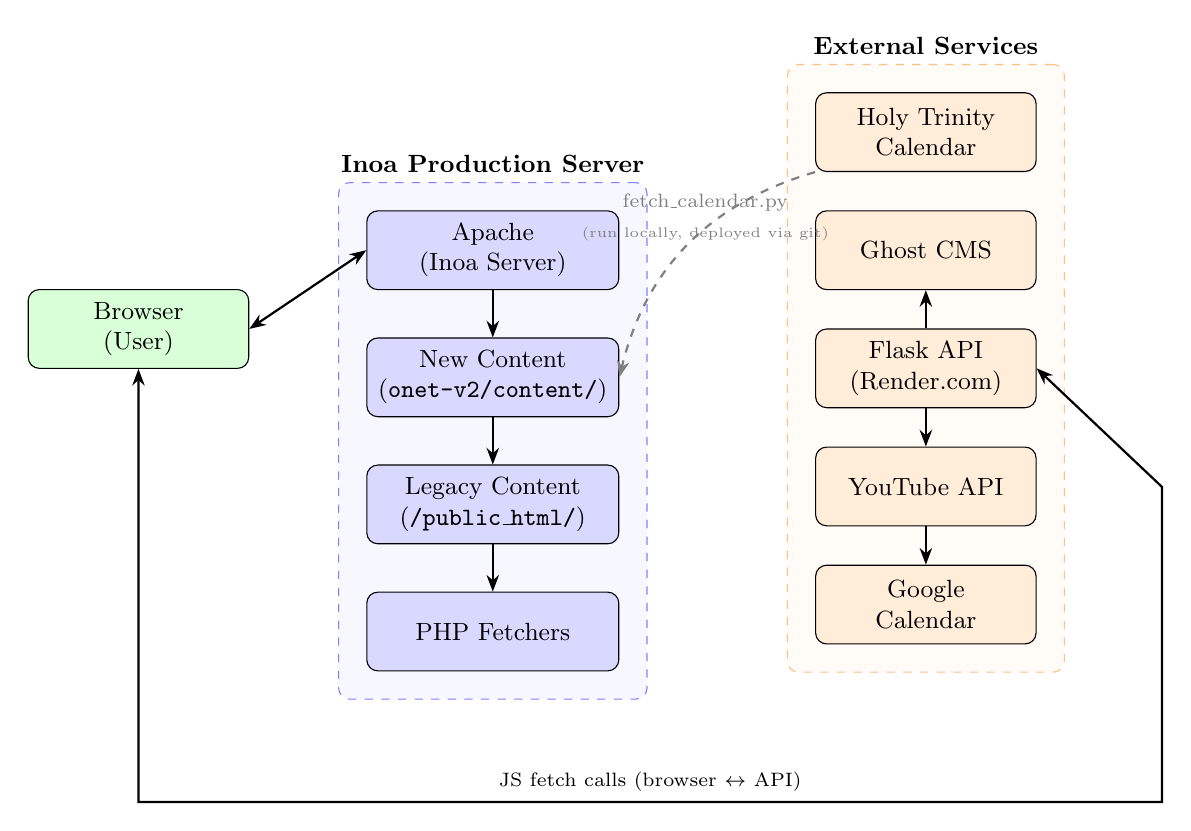
\begin{tikzpicture}[
    box/.style={draw, rounded corners, minimum width=2.8cm, minimum height=1cm, align=center, font=\small},
    serverbox/.style={box, fill=blue!15, minimum width=3.2cm},
    extbox/.style={box, fill=orange!15, minimum width=2.8cm},
    clientbox/.style={box, fill=green!15, minimum width=2.8cm},
    arr/.style={-{Stealth[length=6pt]}, thick},
    darr/.style={{Stealth[length=6pt]}-{Stealth[length=6pt]}, thick},
]

% Client — positioned to the left
\node[clientbox] (browser) at (-4.5, -1) {Browser\\(User)};

% Inoa Server — vertical stack
\node[serverbox] (apache) at (0, 0) {Apache\\(Inoa Server)};
\node[serverbox, below=0.6cm of apache] (newcontent) {New Content\\(\texttt{onet-v2/content/})};
\node[serverbox, below=0.6cm of newcontent] (legacy) {Legacy Content\\(\texttt{/public\_html/})};
\node[serverbox, below=0.6cm of legacy] (php) {PHP Fetchers};

% External Services — to the right, spread vertically
\node[extbox] (holytrin) at (5.5, 1.5) {Holy Trinity\\Calendar};
\node[extbox] (ghost) at (5.5, 0) {Ghost CMS};
\node[extbox] (flask) at (5.5, -1.5) {Flask API\\(Render.com)};
\node[extbox] (youtube) at (5.5, -3) {YouTube API};
\node[extbox] (gcal) at (5.5, -4.5) {Google\\Calendar};

% Arrows — browser to server
\draw[darr] (browser.east) -- (apache.west);

% Arrows — server internal (straight down)
\draw[arr] (apache) -- (newcontent);
\draw[arr] (newcontent) -- (legacy);
\draw[arr] (legacy) -- (php);

% Arrow — browser to Flask API
% Route: down from browser, right under BOTH boxes, then up on the FAR right, then left to Flask
\draw[darr] (browser.south) -- ++(0,-5.5) -- ++(13,0) -- ++(0,4) -- (flask.east);
\node[font=\scriptsize, anchor=north] at (2,-6.5) {JS fetch calls (browser $\leftrightarrow$ API)};

% Arrows — Flask to its services (left side, so they don't conflict with the browser arrow on the right)
\draw[arr] (flask.north) -- (ghost.south);
\draw[arr] (flask.south) -- (youtube.north);
\draw[arr] (youtube.south) -- (gcal.north);

% Arrow — Holy Trinity to new content
% Note: script is run locally, static files are committed and deployed via git
\draw[arr, dashed, gray] (holytrin.south west) to[bend right=30] (newcontent.east);
\node[font=\scriptsize, gray] at (2.7, 0.6) {fetch\_calendar.py};
\node[font=\tiny, gray] at (2.7, 0.2) {(run locally, deployed via git)};

% Background boxes
\begin{scope}[on background layer]
    \node[draw=blue!50, dashed, fill=blue!3, rounded corners, fit=(apache)(newcontent)(legacy)(php), inner sep=10pt, label={[font=\small\bfseries]above:Inoa Production Server}] {};
    \node[draw=orange!50, dashed, fill=orange!3, rounded corners, fit=(holytrin)(ghost)(flask)(youtube)(gcal), inner sep=10pt, label={[font=\small\bfseries]above:External Services}] {};
\end{scope}

\end{tikzpicture}
\caption{System architecture: how the browser, server, and external services interact.}
\label{fig:system-arch}
\end{figure}

\subsection{Repository}

The source code is hosted on GitHub at:

\begin{center}
\url{https://github.com/GZancewicz/onet-v2}
\end{center}

The Flask backend API is a separate repository at:

\begin{center}
\url{https://github.com/GZancewicz/onet-flask-backend}
\end{center}

\subsection{Technology Stack}

\begin{itemize}
    \item \textbf{Markup/Styling}: HTML5, CSS3 (Skeleton grid framework), Google Fonts (Alegreya), Line Awesome icons
    \item \textbf{Client-Side Logic}: Vanilla JavaScript (no frameworks, no build process)
    \item \textbf{Server}: Apache 2.x with \texttt{mod\_rewrite}, minimal PHP for content fetcher scripts
    \item \textbf{Backend API}: Python Flask on Render.com (separate repo)
    \item \textbf{CMS}: Ghost.io (headless, API-only)
    \item \textbf{Utilities}: Python 3 scripts for content processing and maintenance
    \item \textbf{Version Control}: Git, deployed via \texttt{git pull} on production
\end{itemize}

\begin{figure}[ht]
\centering
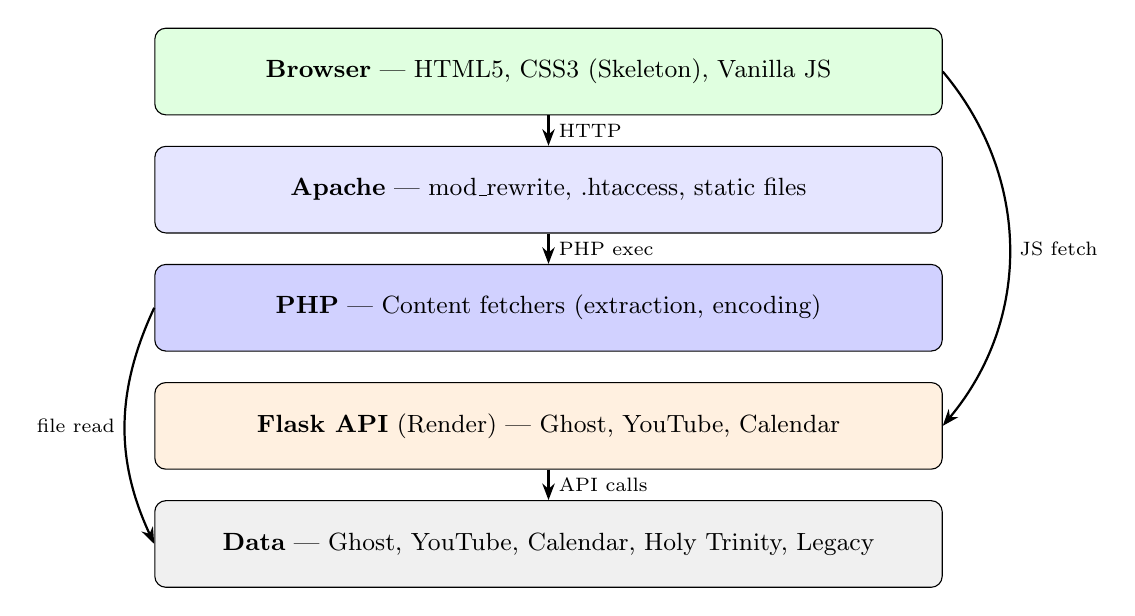
\begin{tikzpicture}[
    layer/.style={draw, rounded corners, minimum width=10cm, minimum height=1.1cm, align=center, font=\small},
    arr/.style={-{Stealth[length=6pt]}, thick},
]

\node[layer, fill=green!12] (client) at (0,0) {\textbf{Browser} --- HTML5, CSS3 (Skeleton), Vanilla JS};
\node[layer, fill=blue!10] (server) at (0,-1.5) {\textbf{Apache} --- mod\_rewrite, .htaccess, static files};
\node[layer, fill=blue!18] (php) at (0,-3.0) {\textbf{PHP} --- Content fetchers (extraction, encoding)};
\node[layer, fill=orange!12] (api) at (0,-4.5) {\textbf{Flask API} (Render) --- Ghost, YouTube, Calendar};
\node[layer, fill=gray!12] (data) at (0,-6.0) {\textbf{Data} --- Ghost, YouTube, Calendar, Holy Trinity, Legacy};

\draw[arr] (client) -- node[right, font=\scriptsize] {HTTP} (server);
\draw[arr] (server) -- node[right, font=\scriptsize] {PHP exec} (php);
\draw[arr] (client.east) to[bend left=40] node[right, font=\scriptsize] {JS fetch} (api.east);
\draw[arr] (api) -- node[right, font=\scriptsize] {API calls} (data);
\draw[arr] (php.west) to[bend right=25] node[left, font=\scriptsize] {file read} (data.west);

\end{tikzpicture}
\caption{Technology stack layers and data flow between them.}
\label{fig:tech-stack}
\end{figure}

\subsection{External Service Dependencies}

\begin{longtable}{p{4cm}p{9cm}}
\toprule
\textbf{Service} & \textbf{Purpose} \\
\midrule
Inoa / Orthodox Internet Services & Production LAMP hosting (cPanel access required) \\
Render.com & Hosts Flask backend API \\
Ghost.io & Headless CMS for articles and blog posts \\
Google Calendar API & Church services and events schedule \\
YouTube Data API v3 & Video content from \texttt{@orthodoxnet} channel \\
Holy Trinity Orthodox & Daily saints and readings calendar data \\
Google Analytics & Site analytics (ID: \texttt{G-D9YEGT19W7}) \\
PayPal SDK & Donation processing \\
\bottomrule
\end{longtable}

\begin{figure}[ht]
\centering
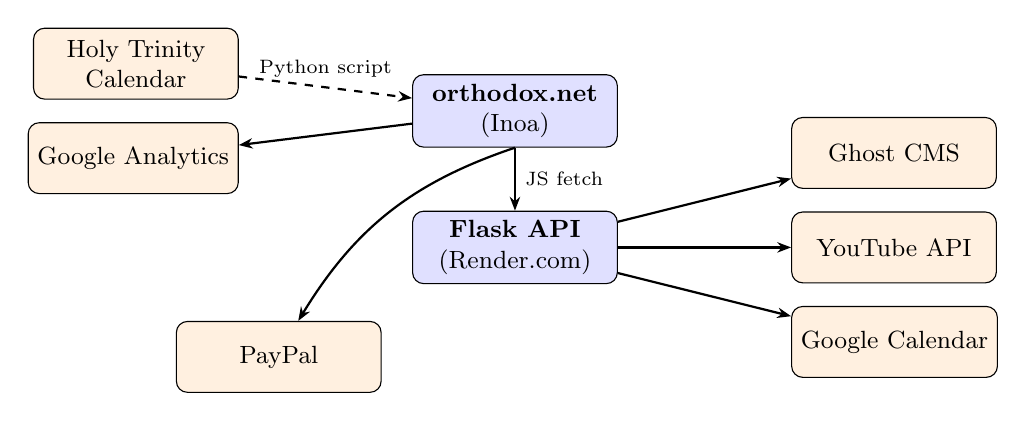
\begin{tikzpicture}[
    svc/.style={draw, rounded corners, minimum width=2.6cm, minimum height=0.9cm, align=center, font=\small, fill=orange!12},
    site/.style={draw, rounded corners, minimum width=2.6cm, minimum height=0.9cm, align=center, font=\small, fill=blue!12},
    arr/.style={-{Stealth[length=5pt]}, thick},
]

\node[site] (site) at (0,0) {\textbf{orthodox.net}\\(Inoa)};
\node[site, below=0.8cm of site] (flask) {\textbf{Flask API}\\(Render.com)};

\node[svc, right=2.2cm of flask, yshift=1.2cm] (ghost) {Ghost CMS};
\node[svc, right=2.2cm of flask] (yt) {YouTube API};
\node[svc, right=2.2cm of flask, yshift=-1.2cm] (gcal) {Google Calendar};

\node[svc, left=2.2cm of site, yshift=0.6cm] (htrin) {Holy Trinity\\Calendar};
\node[svc, left=2.2cm of site, yshift=-0.6cm] (ga) {Google Analytics};
\node[svc, below=2.2cm of site, xshift=-3cm] (paypal) {PayPal};

\draw[arr] (site) -- node[right, font=\scriptsize] {JS fetch} (flask);
\draw[arr] (flask) -- (ghost);
\draw[arr] (flask) -- (yt);
\draw[arr] (flask) -- (gcal);
\draw[arr, dashed] (htrin) -- node[above, font=\scriptsize] {Python script} (site);
\draw[arr] (site) -- (ga);
\draw[arr] (site.south) to[bend right=20] (paypal);

\end{tikzpicture}
\caption{External service dependencies and how they connect to the site.}
\label{fig:ext-services}
\end{figure}

\clearpage
%% ============================================================
\section{Production Server Architecture (Inoa)}
%% ============================================================

\subsection{Server Directory Layout}

The production server is hosted by Inoa/Orthodox Internet Services, accessed via cPanel. The directory structure:

\begin{lstlisting}[language=bash,numbers=none,basicstyle=\ttfamily\scriptsize]
~/public_html/                # Apache DocumentRoot
  .htaccess                   # THE master .htaccess (Section 2.2)
  articles/, sermons/, ...    # ~25 legacy content directories
  new/                        # (no .htaccess here)
    onet-v2/                  # This repository (git clone)
      content/                # Served content
        index.html            # Homepage
        js/, css/, images/    # Static assets
        calendar/data/        # Saints/readings HTML files
        articles/new/         # Shell pages for legacy content
        *.php                 # Content fetcher scripts
      util/                   # Python maintenance scripts
      doc/                    # Documentation
      apache/                 # Reference Apache config files
      legacy/                 # Local testing placeholders
\end{lstlisting}

\textbf{Key observation}: There is \textbf{no} \texttt{.htaccess} in \texttt{/public\_html/new/}. All routing is handled by the single \texttt{.htaccess} in \texttt{/public\_html/}.

Figure~\ref{fig:lamp-filesystem} shows how the \texttt{onet-v2} repository fits into the existing LAMP filesystem on both the production server and the local development environment.

\begin{figure}[ht]
\centering
\resizebox{\textwidth}{!}{%
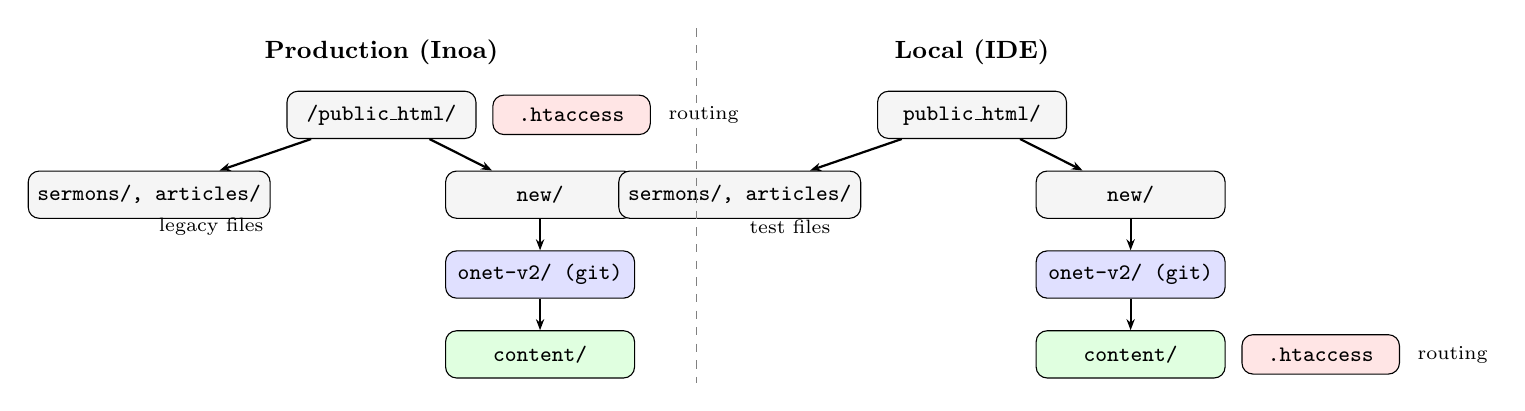
\begin{tikzpicture}[
    dir/.style={draw, rounded corners, minimum width=2.4cm, minimum height=0.6cm, align=center, font=\footnotesize\ttfamily, fill=gray!8},
    repo/.style={draw, rounded corners, minimum width=2.4cm, minimum height=0.6cm, align=center, font=\footnotesize\ttfamily, fill=blue!12},
    htfile/.style={draw, rounded corners, minimum width=2cm, minimum height=0.5cm, align=center, font=\footnotesize\ttfamily, fill=red!10},
    content/.style={draw, rounded corners, minimum width=2.4cm, minimum height=0.6cm, align=center, font=\footnotesize\ttfamily, fill=green!12},
    arr/.style={-{Stealth[length=4pt]}, thick},
    lbl/.style={font=\scriptsize, anchor=west},
    node distance=0.4cm,
]

% Production side
\node[font=\small\bfseries] at (-2.5, 4.2) {Production (Inoa)};
\node[dir] (phtml) at (-2.5, 3.4) {/public\_html/};
\node[htfile, right=0.2cm of phtml] (htprod) {.htaccess};
\node[dir, below left=0.4cm and 0.2cm of phtml] (legacy) {sermons/, articles/};
\node[dir, below right=0.4cm and -0.4cm of phtml] (pnew) {new/};
\node[repo, below=0.4cm of pnew] (ponet) {onet-v2/ (git)};
\node[content, below=0.4cm of ponet] (pcontent) {content/};

\draw[arr] (phtml) -- (legacy);
\draw[arr] (phtml) -- (pnew);
\draw[arr] (pnew) -- (ponet);
\draw[arr] (ponet) -- (pcontent);

\node[lbl] at ($(htprod.east)+(0.1,0)$) {routing};
\node[lbl] at ($(legacy.south)+(0,-0.1)$) {\scriptsize legacy files};

% Local side
\node[font=\small\bfseries] at (5, 4.2) {Local (IDE)};
\node[dir] at (5, 3.4) (lhtml) {public\_html/};
\node[dir, below left=0.4cm and 0.2cm of lhtml] (llegacy) {sermons/, articles/};
\node[dir, below right=0.4cm and -0.4cm of lhtml] (lnew) {new/};
\node[repo, below=0.4cm of lnew] (lonet) {onet-v2/ (git)};
\node[content, below=0.4cm of lonet] (lcontent) {content/};
\node[htfile, right=0.2cm of lcontent] (htdev) {.htaccess};

\draw[arr] (lhtml) -- (llegacy);
\draw[arr] (lhtml) -- (lnew);
\draw[arr] (lnew) -- (lonet);
\draw[arr] (lonet) -- (lcontent);

\node[lbl] at ($(htdev.east)+(0.1,0)$) {routing};
\node[lbl] at ($(llegacy.south)+(0,-0.1)$) {\scriptsize test files};

% Divider
\draw[dashed, gray] (1.5, 4.5) -- (1.5, 0);

\end{tikzpicture}%
}% end resizebox
\caption{The \texttt{onet-v2} repo within the LAMP filesystem.}
\label{fig:lamp-filesystem}
\end{figure}

\subsection{The Production \texttt{.htaccess}}

\textbf{Location on server}: \texttt{\textasciitilde/public\_html/.htaccess}

Figure~\ref{fig:routing-flow} illustrates the routing decision process.

\begin{figure}[ht]
\centering
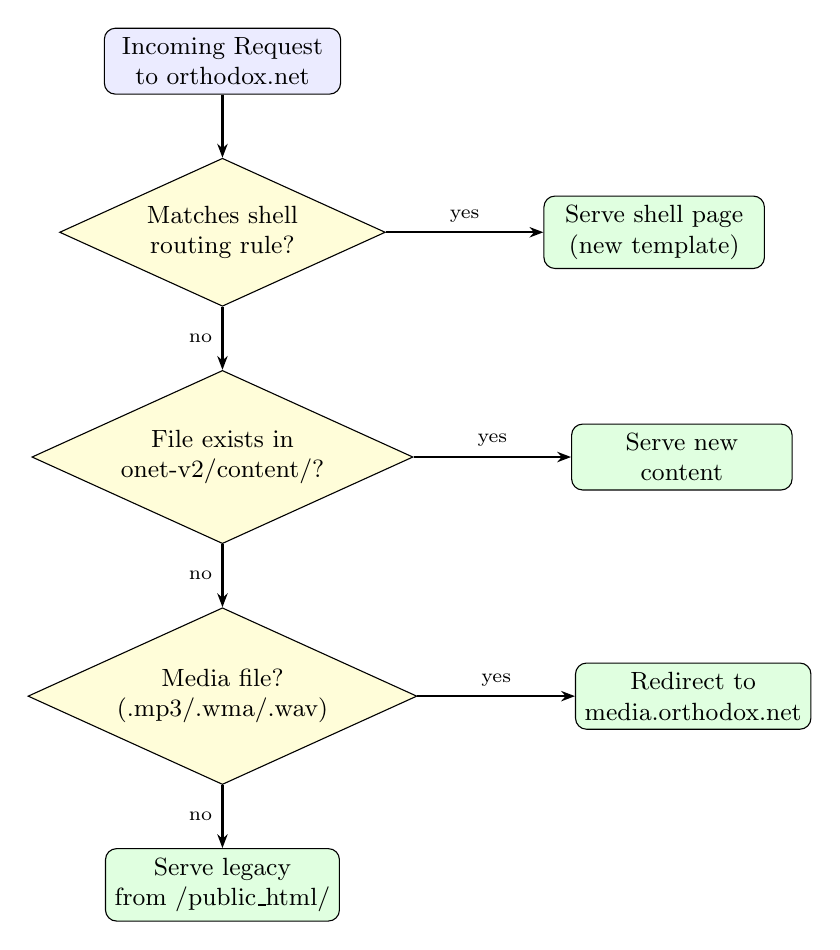
\begin{tikzpicture}[
    block/.style={draw, rounded corners, minimum width=3cm, minimum height=0.8cm, align=center, font=\small, fill=blue!8},
    decision/.style={draw, diamond, aspect=2.2, minimum width=2cm, align=center, font=\small, fill=yellow!15},
    result/.style={draw, rounded corners, minimum width=2.8cm, minimum height=0.8cm, align=center, font=\small, fill=green!12},
    arr/.style={-{Stealth[length=5pt]}, thick},
    node distance=0.7cm,
]

\node[block] (req) {Incoming Request\\to orthodox.net};
\node[decision, below=0.8cm of req] (shell) {Matches shell\\routing rule?};
\node[result, right=2cm of shell] (shellpage) {Serve shell page\\(new template)};
\node[decision, below=0.8cm of shell] (newfile) {File exists in\\onet-v2/content/?};
\node[result, right=2cm of newfile] (newcontent) {Serve new\\content};
\node[decision, below=0.8cm of newfile] (media) {Media file?\\(.mp3/.wma/.wav)};
\node[result, right=2cm of media] (cdn) {Redirect to\\media.orthodox.net};
\node[result, below=0.8cm of media] (legacy) {Serve legacy\\from /public\_html/};

\draw[arr] (req) -- (shell);
\draw[arr] (shell) -- node[above, font=\scriptsize] {yes} (shellpage);
\draw[arr] (shell) -- node[left, font=\scriptsize] {no} (newfile);
\draw[arr] (newfile) -- node[above, font=\scriptsize] {yes} (newcontent);
\draw[arr] (newfile) -- node[left, font=\scriptsize] {no} (media);
\draw[arr] (media) -- node[above, font=\scriptsize] {yes} (cdn);
\draw[arr] (media) -- node[left, font=\scriptsize] {no} (legacy);

\end{tikzpicture}
\caption{Production \texttt{.htaccess} routing decision flow.}
\label{fig:routing-flow}
\end{figure}

This is the single most critical configuration file for the entire site. It is \textbf{not deployed via \texttt{git pull}} and must be \textbf{manually maintained} on the production server. A reference copy is stored in the repository at \texttt{.htaccess.production}, but edits to the production file must be made directly on the server via cPanel File Manager or terminal.

The file combines all routing logic into one place. In order of processing:

\subsubsection{Legacy Folder Shell Routing (lines 7--84)}

These rules intercept requests to legacy content URLs and rewrite them to shell pages that dynamically render the content in the new template. They fire \textbf{before} the content directory check.

\textbf{Pattern}: For each legacy content category, requests to \texttt{/category/filename.html} (excluding \texttt{index.html}) are rewritten to a shell page with an absolute path:

\begin{lstlisting}[language=bash,numbers=none]
RewriteRule ^sermons/(?!index\.html$)([^/]+\.html)$
    /new/onet-v2/content/sermons/new/sermon_shell.html?file=$1 [L,QSA]
\end{lstlisting}

Note the absolute path prefix \texttt{/new/onet-v2/content/} --- this is a critical difference from the local development \texttt{.htaccess} which uses relative paths (see Section~\ref{sec:htaccess-differences}).

Blog posts have a special rule:
\begin{lstlisting}[language=bash,numbers=none]
RewriteRule ^posts/([^/]+)/?$ new_post.html [L]
\end{lstlisting}

\textbf{Mapped categories} (25 total):

{\footnotesize
\begin{longtable}{lll}
\toprule
\textbf{URL Path} & \textbf{Shell Page} & \textbf{PHP Fetcher} \\
\midrule
/articles/ & article\_shell.html & article\_fetcher.php \\
/sermons/ & sermon\_shell.html & sermon\_fetcher.php \\
/scripture/ & scripture\_shell.html & scripture\_fetcher.php \\
/full-voice/ & fullvoice\_shell.html & fullvoice\_fetcher.php \\
/questions/ & questions\_shell.html & questions\_fetcher.php \\
/greatlent/ & greatlent\_shell.html & greatlent\_fetcher.php \\
/pascha/ & pascha\_shell.html & pascha\_fetcher.php \\
/theophany/ & theophany\_shell.html & theophany\_fetcher.php \\
/confess/ & confess\_shell.html & confess\_fetcher.php \\
/fathers/ & fathers\_shell.html & fathers\_fetcher.php \\
/gleanings/ & gleanings\_shell.html & gleanings\_fetcher.php \\
/ustav/ & ustav\_shell.html & ustav\_fetcher.php \\
/services/ & services\_shell.html & services\_fetcher.php \\
/trebnic/ & trebnic\_shell.html & trebnic\_fetcher.php \\
/music/ & music\_shell.html & music\_fetcher.php \\
/menaion-thoughts/ & menaion-thoughts\_shell.html & menaion-thoughts\_fetcher.php \\
/saints/ & saints\_shell.html & saints\_fetcher.php \\
/russiannm/ & russiannm\_shell.html & russiannm\_fetcher.php \\
/links/ & links\_shell.html & links\_fetcher.php \\
/western-saints/ & western-saints\_shell.html & western-saints\_fetcher.php \\
/monastic-stories/ & monastic-stories\_shell.html & monastic-stories\_fetcher.php \\
/poetry/ & poetry\_shell.html & poetry\_fetcher.php \\
/nativity/ & nativity\_shell.html & nativity\_fetcher.php \\
/journal/ & journal\_shell.html & journal\_fetcher.php \\
/posts/* & new\_post.html & (via Flask API) \\
\bottomrule
\end{longtable}
}

\subsubsection{New Content Directory Routing (lines 87--90)}

If no shell routing rule matched, check whether the requested file exists under
\texttt{/new/onet-v2/content/}. If so, serve it from there:

\begin{lstlisting}[language=bash,numbers=none,basicstyle=\ttfamily\footnotesize]
RewriteCond %{DOCUMENT_ROOT}/new/onet-v2/content%{REQUEST_URI} -f [OR]
RewriteCond %{DOCUMENT_ROOT}/new/onet-v2/content%{REQUEST_URI} -d
RewriteRule ^(.*)$ /new/onet-v2/content/$1 [L]
\end{lstlisting}

If the file does \textbf{not} exist in the new content directory, Apache falls through and serves from \texttt{/public\_html/} (legacy content). This is the core mechanism enabling progressive migration.

\subsubsection{Media CDN Redirect (lines 93--98)}

MP3, WMA, and WAV files are redirected to \texttt{media.orthodox.net}:

\begin{lstlisting}[language=bash,numbers=none]
RewriteCond %{HTTP_HOST} ^(www\.)?orthodox\.net [NC]
RewriteRule (.*).mp3 http://media.orthodox.net/$1.mp3 [L]
RewriteRule (.*).wma http://media.orthodox.net/$1.wma [L]
RewriteRule (.*).wav http://media.orthodox.net/$1.wav [L]
\end{lstlisting}

\subsubsection{URL Normalization (lines 103--140)}

Forces all URLs to lowercase via character-by-character replacement with 301 permanent redirects. Excludes cPanel DCV validation and ACME challenge paths.

\subsubsection{Server Configuration (lines 142--167)}

\begin{itemize}
    \item \texttt{ErrorDocument 404 /cgi-bin/404.pl} --- custom Perl 404 handler
    \item \texttt{AddType "text/html;charset=windows-1251"} for \texttt{.shtml}, \texttt{.html}, \texttt{.htm} --- legacy charset
    \item Media MIME types for legacy Windows Media formats (ASF, WMA, WMV, etc.)
    \item PHP handler: \texttt{ea-php82} via cPanel
    \item \texttt{ModPagespeed unplugged} --- disables Google PageSpeed module
\end{itemize}

\subsection{Adding a New Legacy Folder Conversion}

When migrating a new legacy content category:

\begin{enumerate}
    \item Create the shell HTML page at \texttt{content/CATEGORY/new/CATEGORY\_shell.html}
    \item Create the PHP fetcher at \texttt{content/CATEGORY\_fetcher.php}
    \item Create the JavaScript shell script at \texttt{content/js/CATEGORY-shell.js}
    \item Add a RewriteRule to the \textbf{production} \texttt{.htaccess} at \texttt{\textasciitilde/public\_html/.htaccess} (manually, via cPanel)
    \item Add the same rule (with relative paths) to \texttt{content/.htaccess} in the repo for local development
    \item Commit and deploy the new files via \texttt{git pull}
\end{enumerate}

%% ============================================================
\section{\texttt{.htaccess} Management: Local vs.\ Production}
\label{sec:htaccess-differences}
%% ============================================================

This is one of the most important operational details for this project. The \texttt{.htaccess} files that control URL routing are \textbf{different between local development and production}, and the production file is \textbf{not managed by git}.

\begin{figure}[ht]
\centering
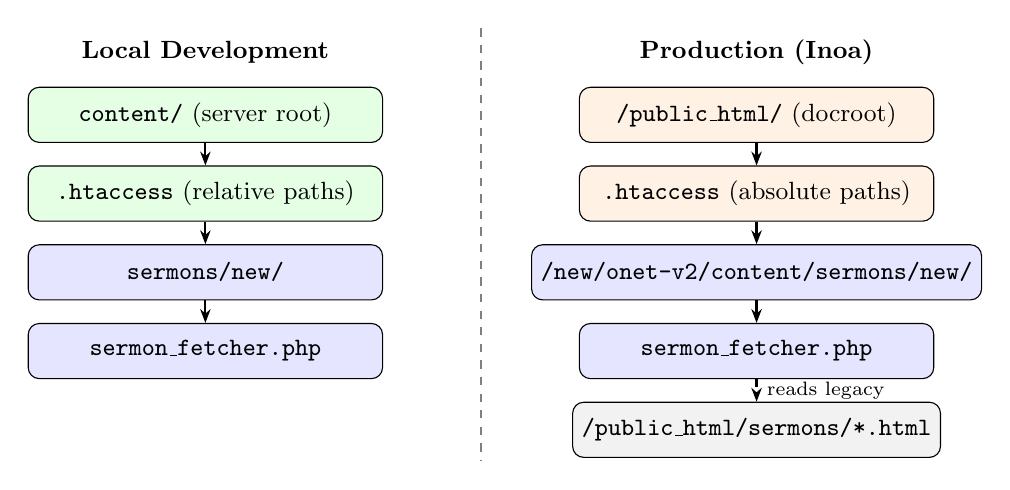
\begin{tikzpicture}[
    box/.style={draw, rounded corners, minimum width=4.5cm, minimum height=0.7cm, align=center, font=\small},
    lbl/.style={font=\small\bfseries, align=center},
    arr/.style={-{Stealth[length=5pt]}, thick},
]

% LOCAL side
\node[lbl] (ltitle) at (-3.5, 3) {Local Development};
\node[box, fill=green!10] (lroot) at (-3.5, 2.2) {\texttt{content/} (server root)};
\node[box, fill=green!10] (lhtaccess) at (-3.5, 1.2) {\texttt{.htaccess} (relative paths)};
\node[box, fill=blue!10] (lshell) at (-3.5, 0.2) {\texttt{sermons/new/}};
\node[box, fill=blue!10] (lfetcher) at (-3.5, -0.8) {\texttt{sermon\_fetcher.php}};

\draw[arr] (lroot) -- (lhtaccess);
\draw[arr] (lhtaccess) -- (lshell);
\draw[arr] (lshell) -- (lfetcher);

% PRODUCTION side
\node[lbl] (ptitle) at (3.5, 3) {Production (Inoa)};
\node[box, fill=orange!10] (proot) at (3.5, 2.2) {\texttt{/public\_html/} (docroot)};
\node[box, fill=orange!10] (phtaccess) at (3.5, 1.2) {\texttt{.htaccess} (absolute paths)};
\node[box, fill=blue!10] (pshell) at (3.5, 0.2) {\texttt{/new/onet-v2/content/sermons/new/}};
\node[box, fill=blue!10] (pfetcher) at (3.5, -0.8) {\texttt{sermon\_fetcher.php}};
\node[box, fill=gray!10] (plegacy) at (3.5, -1.8) {\texttt{/public\_html/sermons/*.html}};

\draw[arr] (proot) -- (phtaccess);
\draw[arr] (phtaccess) -- (pshell);
\draw[arr] (pshell) -- (pfetcher);
\draw[arr, dashed] (pfetcher) -- node[right, font=\scriptsize] {reads legacy} (plegacy);

% Divider
\draw[dashed, gray] (0, 3.3) -- (0, -2.2);

\end{tikzpicture}
\caption{Side-by-side comparison of local vs.\ production path resolution.}
\label{fig:local-vs-prod}
\end{figure}

\subsection{Why They Differ}

On the production server (Inoa), the Apache DocumentRoot is \texttt{/public\_html/}. The new site content lives several directories deep at \texttt{/public\_html/new/onet-v2/content/}. Shell routing rules must use absolute paths from the DocumentRoot:

\begin{lstlisting}[language=bash,numbers=none]
# PRODUCTION: absolute path from /public_html/
RewriteRule ^sermons/(?!index\.html$)([^/]+\.html)$
    /new/onet-v2/content/sermons/new/sermon_shell.html?file=$1 [L,QSA]
\end{lstlisting}

Locally (using \texttt{php -S localhost:8000} from the \texttt{content/} directory), the server root \emph{is} the content directory, so rules use relative paths:

\begin{lstlisting}[language=bash,numbers=none]
# LOCAL: relative path (content/ is the server root)
RewriteRule ^sermons/(?!index\.html$)([^/]+\.html)$
    sermons/new/sermon_shell.html?file=$1 [L,QSA]
\end{lstlisting}

\subsection{File Inventory}

\begin{longtable}{p{4.8cm}p{8cm}}
\toprule
\textbf{File in Repo} & \textbf{Purpose} \\
\midrule
\texttt{content/.htaccess} & \textbf{Local development} version. Uses relative paths. Checked into git. Used when running \texttt{php -S} from \texttt{content/}. \\
\midrule
\texttt{.htaccess.production} & \textbf{Reference copy} of what should be on the production server at \texttt{\textasciitilde/public\_html/.htaccess}. Uses absolute paths. Checked into git but \textbf{not automatically deployed}. \\
\midrule
\texttt{apache/.htaccess} & Reference copy of the primary rewrite rules (content routing, CDN, URL normalization). Used as basis for the production file. \\
\midrule
\texttt{apache/.htaccess.inoa} & Historical: older Inoa config using symlinks (\texttt{/onet/}, \texttt{/parent/}). Superseded. \\
\midrule
\texttt{apache/.htaccess\_v1} & Historical: earlier version without content directory routing. \\
\midrule
\tpath{apache/public\_html/\allowbreak .htaccess} & Reference copy of production \texttt{.htaccess} with both shell routing and content routing combined. \\
\midrule
\texttt{apache/httpd.conf} & Local Apache config for macOS (Homebrew). Points DocumentRoot to \texttt{content/}. \\
\bottomrule
\end{longtable}

\subsection{Critical Operational Rule}

\begin{center}
\fbox{\parbox{0.88\textwidth}{
\textbf{When you add or modify a shell routing rule}, update \textbf{both}:
\begin{enumerate}
    \item \texttt{content/.htaccess} in the repo (relative paths, local dev)
    \item \texttt{\textasciitilde/public\_html/.htaccess} on Inoa (absolute paths, via cPanel)
\end{enumerate}
Keep \texttt{.htaccess.production} in the repo as a reference copy.

\texttt{git pull} does \textbf{not} update the production \texttt{.htaccess}.
}}
\end{center}

\subsection{Verifying the Production \texttt{.htaccess}}

The production file includes a test redirect at the top:

\begin{lstlisting}[language=bash,numbers=none,basicstyle=\ttfamily\scriptsize]
Redirect 302 /test-htaccess-check /test-htaccess-check-success
\end{lstlisting}

To verify the \texttt{.htaccess} is active, visit\\
\texttt{https://orthodox.net/test-htaccess-check}\\
in a browser. If it redirects to \texttt{/test-htaccess-check-success}, the file is active.

%% ============================================================
\section{Legacy Content Migration System}
%% ============================================================

The legacy migration system is the most architecturally significant part of the codebase. It allows legacy HTML pages (some dating back 20+ years, many exported from Microsoft Word) to be served through the new site template without modifying the original files.

\subsection{Request Flow (Production)}

Figure~\ref{fig:legacy-flow} illustrates the complete request lifecycle for legacy content.

\begin{figure}[ht]
\centering
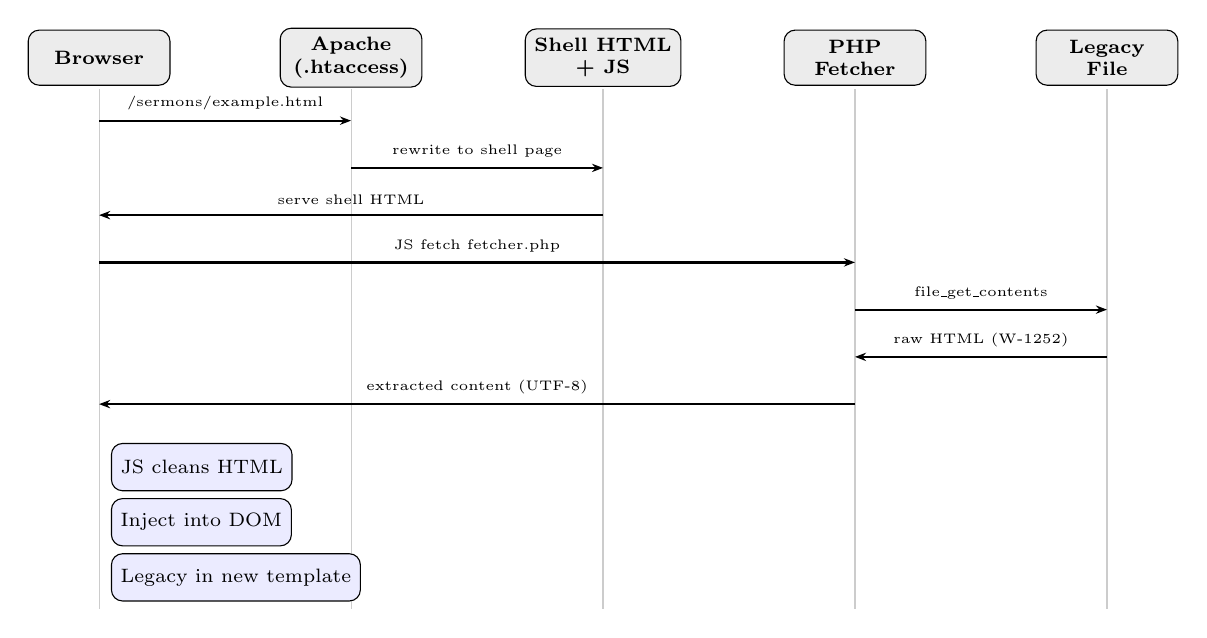
\begin{tikzpicture}[
    actor/.style={draw, rounded corners, minimum width=1.8cm, minimum height=0.7cm, align=center, font=\scriptsize\bfseries, fill=gray!15},
    stepbox/.style={draw, rounded corners, minimum width=2.2cm, minimum height=0.6cm, align=center, font=\scriptsize, fill=blue!8},
    arr/.style={-{Stealth[length=4pt]}, thick},
    node distance=0.15cm,
]

% Actors across the top
\node[actor] (browser) at (0, 0) {Browser};
\node[actor] (apache) at (3.2, 0) {Apache\\(.htaccess)};
\node[actor] (shell) at (6.4, 0) {Shell HTML\\+ JS};
\node[actor] (php) at (9.6, 0) {PHP\\Fetcher};
\node[actor] (legacy) at (12.8, 0) {Legacy\\File};

% Vertical lifelines
\foreach \x in {0, 3.2, 6.4, 9.6, 12.8} {
    \draw[gray!40] (\x, -0.4) -- (\x, -7);
}

% Sequence steps
\draw[arr] (0, -0.8) -- node[above, font=\tiny] {/sermons/example.html} (3.2, -0.8);
\draw[arr] (3.2, -1.4) -- node[above, font=\tiny] {rewrite to shell page} (6.4, -1.4);
\draw[arr] (6.4, -2.0) -- node[above, font=\tiny] {serve shell HTML} (0, -2.0);
\draw[arr] (0, -2.6) -- node[above, font=\tiny] {JS fetch fetcher.php} (9.6, -2.6);
\draw[arr] (9.6, -3.2) -- node[above, font=\tiny] {file\_get\_contents} (12.8, -3.2);
\draw[arr] (12.8, -3.8) -- node[above, font=\tiny] {raw HTML (W-1252)} (9.6, -3.8);
\draw[arr] (9.6, -4.4) -- node[above, font=\tiny] {extracted content (UTF-8)} (0, -4.4);

% Browser processing
\node[stepbox, anchor=west] at (0.15, -5.2) {JS cleans HTML};
\node[stepbox, anchor=west] at (0.15, -5.9) {Inject into DOM};
\node[stepbox, anchor=west] at (0.15, -6.6) {Legacy in new template};

\end{tikzpicture}
\caption{Sequence diagram: legacy content request lifecycle on production.}
\label{fig:legacy-flow}
\end{figure}

\begin{enumerate}
    \item User requests \texttt{https://orthodox.net/sermons/example.html}
    \item Apache reads \texttt{/public\_html/.htaccess}
    \item Shell routing rule rewrites to\\
    \texttt{/new/onet-v2/content/sermons/new/sermon\_shell.html?file=example.html}
    \item \texttt{sermon\_shell.html} loads \texttt{sermon-shell.js}
    \item JavaScript extracts \texttt{file=example.html} from the query string
    \item JavaScript fetches \texttt{/sermon\_fetcher.php?file=example.html}
    \item PHP reads \texttt{/public\_html/sermons/example.html} from disk
    \item PHP extracts content between \texttt{<!--BEGIN-CONTENT-->} and \texttt{<!--END-CONTENT-->} markers
    \item PHP converts encoding from Windows-1252 to UTF-8
    \item JavaScript receives HTML, cleans Microsoft Word artifacts, normalizes paths
    \item JavaScript injects cleaned HTML into \texttt{\#sermon-placeholder} div
    \item Result: legacy content displayed within the modern site template
\end{enumerate}

\subsection{PHP Content Fetchers}

All fetcher scripts follow the same pattern. Using \texttt{sermon\_fetcher.php} as the canonical example:

\begin{lstlisting}[language=PHP,caption={sermon\_fetcher.php (representative pattern)}]
<?php
header('Content-Type: text/html; charset=utf-8');
mb_internal_encoding('UTF-8');

if (!isset($_GET['file'])) {
    http_response_code(400);
    echo "Missing file parameter.";
    exit;
}

// Security: basename() prevents directory traversal
$filename = basename($_GET['file']);
$filepath = __DIR__ . '/../../../../public_html/sermons/' . $filename;

if (!file_exists($filepath)) {
    http_response_code(404);
    echo "File not found.";
    exit;
}

$content = file_get_contents($filepath);
// Convert legacy Windows-1252 encoding to UTF-8
$content = mb_convert_encoding($content, 'UTF-8', 'Windows-1252');

// Extract content between markers
if (preg_match(
    '/<!--BEGIN-CONTENT-->[\s\r\n]*(.*?)[\s\r\n]*<!--END-CONTENT-->/is',
    $content, $matches)) {
    echo $matches[1];
} else {
    echo $content; // Fallback: serve entire file
}
?>
\end{lstlisting}

\textbf{Security}: All fetchers use \texttt{basename()} to strip directory components, preventing path traversal attacks.

\textbf{Encoding}: Legacy files use Windows-1252 encoding. Fetchers convert to UTF-8 before returning to the browser.

\textbf{Content Markers}: Legacy pages use \texttt{<!--BEGIN-CONTENT-->} and \texttt{<!--END-CONTENT-->} HTML comments to delimit the main content area. If markers are absent, the entire file is returned.

\textbf{File Path}: The relative path \texttt{\_\_DIR\_\_ . '/../../../../public\_html/'} traverses from \texttt{content/} up to the server root. This path is correct on the Inoa production server. Locally, it depends on your directory structure matching the expected layout.

\subsection{JavaScript Shell Scripts}

Each shell script handles client-side content cleaning. The \texttt{article-shell.js} pattern:

\begin{lstlisting}[language=JavaScript,caption={Shell script pattern (article-shell.js)}]
document.addEventListener('DOMContentLoaded', function() {
    // Extract filename from query string or URL path
    const urlParams = new URLSearchParams(window.location.search);
    let file = urlParams.get('file');
    if (!file) {
        const match = window.location.pathname.match(/\/([^\/]+\.html)$/);
        if (match) file = match[1];
    }

    fetch(`/article_fetcher.php?file=${encodeURIComponent(file)}`)
        .then(response => response.text())
        .then(html => {
            const parser = new DOMParser();
            const doc = parser.parseFromString(html, 'text/html');

            // Convert all headings to h4
            doc.querySelectorAll('h1,h2,h3,h5,h6')
               .forEach(h => { /* convert to h4 */ });

            // Normalize relative paths to absolute
            doc.querySelectorAll('img').forEach(img => {
                if (img.src && !img.src.startsWith('http')) {
                    img.src = 'https://www.orthodox.net/articles/' + img.src;
                }
            });

            document.getElementById('article-placeholder')
                    .innerHTML = doc.body.innerHTML;
        });
});
\end{lstlisting}

\textbf{Sermon-specific cleaning} (\texttt{sermon-shell.js}) additionally:
\begin{itemize}
    \item Removes Microsoft Word CSS classes: \texttt{MsoBodyText},\\ \texttt{MsoFootnoteText}, \texttt{MsoHeader}
    \item Strips all \texttt{<style>} tags and inline \texttt{style} attributes
    \item Converts \texttt{p.MsoHeader} elements to semantic heading tags
    \item Normalizes media file links (jpg, mp3, pdf) to absolute URLs at\\ \texttt{https://www.orthodox.net/sermons/}
\end{itemize}

%% ============================================================
\section{Frontend Architecture}
%% ============================================================

\subsection{HTML Template Structure}

All pages share a common template maintained by \texttt{util/update\_template.py}. The template (\texttt{util/template.html}) defines the HTML \texttt{<head>} section:

\begin{itemize}
    \item Meta tags (charset, viewport, CSP, description, keywords, OpenGraph)
    \item CSS imports (Skeleton, custom stylesheets, icon fonts)
    \item Analytics and PayPal SDK scripts
\end{itemize}

The body structure across all pages:

\begin{lstlisting}[language=HTML,numbers=none]
<div class="section section-banner">
    <!-- Church logo, title, subtitle -->
</div>
<div class="navBar-section" id="navbar">
    <!-- Navigation links, hamburger menu -->
</div>
<div class="section section-main" id="page-content">
    <!-- Page-specific content -->
</div>
<div class="section section-other-links">
    <!-- Footer links -->
</div>
\end{lstlisting}

\subsection{CSS Architecture}

\subsubsection{Skeleton Framework}

The site uses Skeleton CSS (\texttt{/css/skeleton.css}), a lightweight responsive grid system with a 12-column layout. Skeleton provides base typography and a mobile-first responsive grid.

\subsubsection{Custom Stylesheets}

\begin{longtable}{p{3.5cm}p{3cm}p{6.5cm}}
\toprule
\textbf{File} & \textbf{Version} & \textbf{Purpose} \\
\midrule
\texttt{style.css} & \texttt{?v=14} & Primary site styles: colors, typography, section layout \\
\texttt{nav.css} & -- & Navigation bar: desktop float layout, mobile hamburger \\
\texttt{calendar.css} & -- & Holy Trinity calendar content styling \\
\texttt{normalize.css} & -- & Browser reset (bundled with Skeleton) \\
\texttt{dropdown.css} & -- & Dropdown menu styling \\
\bottomrule
\end{longtable}

\subsubsection{Design Tokens}

Key values from \texttt{style.css}:

\begin{longtable}{p{4cm}p{4cm}p{5cm}}
\toprule
\textbf{Property} & \textbf{Value} & \textbf{Usage} \\
\midrule
Background & \texttt{\#f2e1c5} & Page background (cream) \\
Link color & \texttt{\#1c5880} & All anchor tags (dark blue) \\
Banner title & \texttt{\#850f00} & Church name heading (dark red) \\
Banner subtitle & \texttt{\#1c5880} & Subtitle text (dark blue) \\
Nav background & \texttt{darkslategray} & Navigation bar (opacity 0.8) \\
Nav hover & \texttt{\#009cde} text on white bg & Navigation link hover state \\
Base font size & \texttt{75\%} & HTML root element \\
Font family & Alegreya, serif & Primary typeface (Google Fonts) \\
\bottomrule
\end{longtable}

\subsubsection{Responsive Breakpoints}

\begin{longtable}{p{4cm}p{9cm}}
\toprule
\textbf{Breakpoint} & \textbf{Behavior} \\
\midrule
$\leq$ 550px & Video thumbnails shrink to 160px width \\
$\leq$ 700px & Hamburger menu activates; nav links collapse; video thumbnails 260px \\
$\leq$ 900px & Video thumbnails reduce to 320px width \\
$>$ 700px & Full horizontal navigation bar; video thumbnails at 400px \\
\bottomrule
\end{longtable}

\subsection{JavaScript Architecture}

Figure~\ref{fig:homepage-arch} shows how the homepage JavaScript files connect to APIs and DOM elements.

\begin{figure}[ht]
\centering
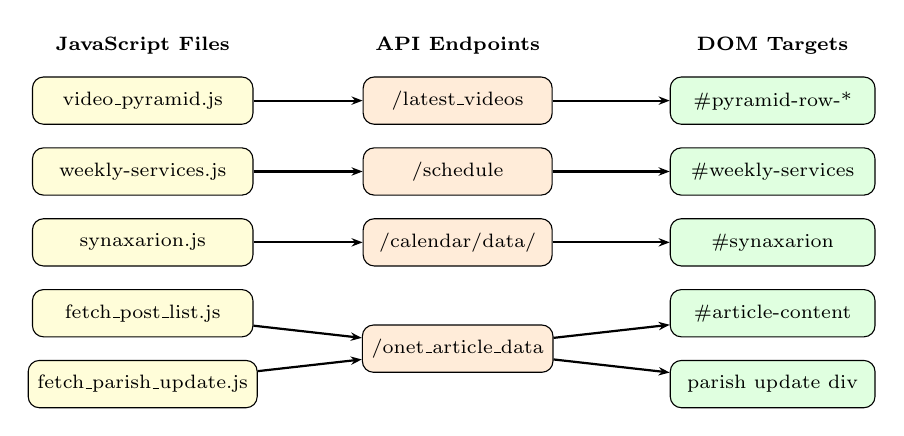
\begin{tikzpicture}[
    js/.style={draw, rounded corners, minimum width=2.8cm, minimum height=0.6cm, align=center, font=\scriptsize, fill=yellow!15},
    api/.style={draw, rounded corners, minimum width=2.4cm, minimum height=0.6cm, align=center, font=\scriptsize, fill=orange!15},
    dom/.style={draw, rounded corners, minimum width=2.6cm, minimum height=0.6cm, align=center, font=\scriptsize, fill=green!12},
    lbl/.style={font=\scriptsize\bfseries},
    arr/.style={-{Stealth[length=4pt]}, thick},
]

% Column labels
\node[lbl] at (-4, 2.5) {JavaScript Files};
\node[lbl] at (0, 2.5) {API Endpoints};
\node[lbl] at (4, 2.5) {DOM Targets};

% JS files
\node[js] (vp) at (-4, 1.8) {video\_pyramid.js};
\node[js] (ws) at (-4, 0.9) {weekly-services.js};
\node[js] (syn) at (-4, 0) {synaxarion.js};
\node[js] (fpl) at (-4, -0.9) {fetch\_post\_list.js};
\node[js] (fpu) at (-4, -1.8) {fetch\_parish\_update.js};

% API endpoints
\node[api] (lv) at (0, 1.8) {/latest\_videos};
\node[api] (sched) at (0, 0.9) {/schedule};
\node[api] (local) at (0, 0) {/calendar/data/};
\node[api] (oad) at (0, -1.35) {/onet\_article\_data};

% DOM targets
\node[dom] (dpyr) at (4, 1.8) {\#pyramid-row-*};
\node[dom] (dws) at (4, 0.9) {\#weekly-services};
\node[dom] (dsyn) at (4, 0) {\#synaxarion};
\node[dom] (dart) at (4, -0.9) {\#article-content};
\node[dom] (dpar) at (4, -1.8) {parish update div};

% Arrows
\draw[arr] (vp) -- (lv);   \draw[arr] (lv) -- (dpyr);
\draw[arr] (ws) -- (sched); \draw[arr] (sched) -- (dws);
\draw[arr] (syn) -- (local); \draw[arr] (local) -- (dsyn);
\draw[arr] (fpl) -- (oad);  \draw[arr] (oad) -- (dart);
\draw[arr] (fpu) -- (oad);  \draw[arr] (oad) -- (dpar);

\end{tikzpicture}
\caption{Homepage: JavaScript files, API endpoints, and DOM injection targets.}
\label{fig:homepage-arch}
\end{figure}

There is no build system, bundler, or transpiler. All JavaScript files are vanilla ES5/ES6 loaded via \texttt{<script>} tags with query-string cache busting (\texttt{?v=N}).

\subsubsection{Configuration}

\begin{lstlisting}[language=JavaScript,caption={/content/js/config.js}]
const CONFIG = {
    VERSION: '2',
    FLASK_BACKEND_URL:
        'https://production-orthodox-net-flask.onrender.com'
};
\end{lstlisting}

All scripts that call the backend API reference \texttt{CONFIG.FLASK\_BACKEND\_URL}. This file \textbf{must} be included before any API-calling script:

\begin{lstlisting}[language=HTML,numbers=none]
<script src="/js/config.js?v=2"></script>
<script src="/js/fetch_article.js?v=1"></script>
\end{lstlisting}

\subsubsection{Page-Level Cache Busting}

The homepage (\texttt{index.html}) implements a page-level cache buster via \texttt{localStorage}:

\begin{lstlisting}[language=JavaScript,numbers=none]
const PAGE_VERSION = '20241202a';
if (localStorage.getItem('pageVersion') !== PAGE_VERSION) {
    localStorage.setItem('pageVersion', PAGE_VERSION);
    window.location.reload(true);
}
\end{lstlisting}

Format: \texttt{YYYYMMDDx} where \texttt{x} is a letter suffix for same-day updates.

\subsubsection{JavaScript File Reference}

\paragraph{Core/Infrastructure}

\begin{longtable}{p{4.5cm}p{8cm}}
\toprule
\textbf{File} & \textbf{Purpose} \\
\midrule
\texttt{config.js} & API base URL and version constant \\
\texttt{navbar.js} & Hamburger menu toggle; listens on \texttt{.icon} click, toggles \texttt{.responsive} class on \texttt{\#mainNavBar} \\
\texttt{gtag.js} & Google Analytics initialization \\
\texttt{ppal.js} & PayPal donation form integration \\
\texttt{analytics.js} & (Deprecated/empty) \\
\bottomrule
\end{longtable}

\paragraph{Homepage Dynamic Content}

{\small
\begin{longtable}{p{4.5cm}p{3.5cm}p{4.5cm}}
\toprule
\textbf{File} & \textbf{API Endpoint} & \textbf{Target DOM Element} \\
\midrule
\texttt{video\_pyramid.js} & \texttt{/latest\_videos} & \texttt{\#pyramid-row-1} through \texttt{\#pyramid-row-5} \\
\texttt{weekly-services.js} & \texttt{/schedule} & \texttt{\#weekly-services} \\
\texttt{synaxarion.js} & Local file & \texttt{\#synaxarion} \\
\texttt{fetch\_post\_list.js} & \texttt{/onet\_article\_data} & \texttt{\#article-content} \\
\texttt{fetch\_parish\_update.js} & \texttt{/onet\_article\_data} & Parish update section \\
\bottomrule
\end{longtable}
}

\paragraph{CMS Content Scripts}

{\footnotesize
\begin{longtable}{lll}
\toprule
\textbf{File} & \textbf{API Endpoint} & \textbf{Target DOM} \\
\midrule
\texttt{fetch\_article.js} & \texttt{/onet\_article} & \texttt{\#article-content} \\
\texttt{fetch\_all\_posts.js} & \texttt{/onet\_article\_data} & Post listing \\
\texttt{fetch\_article\_list.js} & \texttt{/onet\_articles\_to\_list} & Article listing \\
\texttt{fetch\_article\_by\_slug.js} & \texttt{/onet\_article} & Article content \\
\texttt{fetch\_latest\_article.js} & \texttt{/onet\_article\_data} & Latest article \\
\texttt{fetch\_post.js} & \texttt{/onet\_article} & \texttt{\#article-content} \\
\texttt{fetch\_motd.js} & \texttt{/onet\_article\_data} & Message of the day \\
\texttt{fetch\_parish\_life.js} & \texttt{/parish\_life} & Parish life section \\
\texttt{show-legacy-article.js} & \texttt{/legacy\_article} & Legacy article display \\
\texttt{fetch\_legacy\_article.js} & \texttt{/legacy\_article} & Legacy content \\
{\footnotesize\texttt{fetch\_legacy\_article\_from\_cms.js}} & \texttt{/legacy\_article} & Legacy via CMS \\
\bottomrule
\end{longtable}
}

\paragraph{Legacy Folder Shell Scripts (22 files)}

All \texttt{*-shell.js} files follow the pattern described in Section~4.3. Each corresponds to a legacy content category and its PHP fetcher.

\paragraph{Specialized Scripts}

{\small
\begin{longtable}{p{4.8cm}p{7.7cm}}
\toprule
\textbf{File} & \textbf{Purpose} \\
\midrule
\texttt{catechism.js} & Catechism page interactivity \\
\texttt{catechism-qa.js} & Catechism Q\&A accordion/toggle behavior \\
\texttt{carousel\_main.js} & YouTube video carousel (homepage variant) \\
\texttt{format-bible-verses.js} & Formats inline Bible verse references \\
\texttt{gleanings-categories.js} & Gleanings content category filtering \\
\texttt{gleanings-topics.js} & Gleanings topic-based navigation \\
\texttt{change-url.js} & URL manipulation utility \\
\texttt{change-blog-url.js} & Blog URL formatting \\
\texttt{content-html.js} & Generic content HTML processing \\
\texttt{blog.js} & Blog page functionality \\
\texttt{calendar.js} & Calendar page display \\
\texttt{homilies.js} & Homilies listing \\
\texttt{latest-homily.js} & Latest homily display \\
\texttt{loadCalendar2.js} & Alternate calendar loader \\
\bottomrule
\end{longtable}
}

%% ============================================================
\section{Synaxarion (Saints \& Readings)}
%% ============================================================

The ``Today's Saints \& Readings'' section on the homepage uses pre-generated static HTML files rather than a live API call, for performance. Figure~\ref{fig:synaxarion-flow} illustrates the two-phase data flow.

\begin{figure}[ht]
\centering
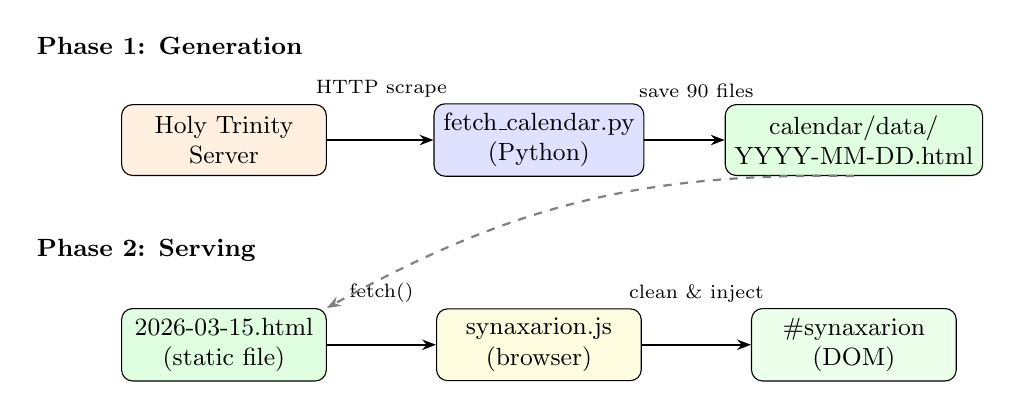
\begin{tikzpicture}[
    box/.style={draw, rounded corners, minimum width=2.6cm, minimum height=0.9cm, align=center, font=\small},
    arr/.style={-{Stealth[length=5pt]}, thick},
    lbl/.style={font=\scriptsize, fill=white, inner sep=1pt},
]

% Phase 1: Generation (top row)
\node[font=\small\bfseries, anchor=west] at (-5.5, 2.2) {Phase 1: Generation};
\node[box, fill=orange!12] (ht) at (-3, 1) {Holy Trinity\\Server};
\node[box, fill=blue!12] (script) at (1, 1) {fetch\_calendar.py\\(Python)};
\node[box, fill=green!12] (files) at (5, 1) {calendar/data/\\YYYY-MM-DD.html};

\draw[arr] (ht) -- (script);
\node[lbl, above] at (-1, 1.5) {HTTP scrape};
\draw[arr] (script) -- (files);
\node[lbl, above] at (3, 1.5) {save 90 files};

% Phase 2: Serving (bottom row)
\node[font=\small\bfseries, anchor=west] at (-5.5, -0.4) {Phase 2: Serving};
\node[box, fill=green!12] (files2) at (-3, -1.6) {2026-03-15.html\\(static file)};
\node[box, fill=yellow!12] (synjs) at (1, -1.6) {synaxarion.js\\(browser)};
\node[box, fill=green!8] (dom) at (5, -1.6) {\#synaxarion\\(DOM)};

\draw[arr] (files2) -- (synjs);
\node[lbl, above] at (-1, -1.1) {fetch()};
\draw[arr] (synjs) -- (dom);
\node[lbl, above] at (3, -1.1) {clean \& inject};

% Connection between phases
\draw[arr, dashed, gray] (files.south) to[bend right=15] (files2.north east);

\end{tikzpicture}
\caption{Synaxarion data flow: pre-generation (offline) and serving (runtime).}
\label{fig:synaxarion-flow}
\end{figure}

\subsection{Data Source}

Calendar data is scraped from Holy Trinity Russian Orthodox Church:

\begin{lstlisting}[language=bash,numbers=none]
https://www.holytrinityorthodox.com/calendar/doc/examples/ppp.php
    ?month=MM&today=DD&year=YYYY
    &dt=1&header=1&lives=1&trp=1&scripture=1
    &sid=RANDOM
\end{lstlisting}

\subsection{Data Files}

Files are stored at \texttt{/content/calendar/data/YYYY-MM-DD.html}. Each file contains the saints, scripture readings, and troparion for that date.

\subsection{Client-Side Loading (\texttt{synaxarion.js})}

\begin{enumerate}
    \item Computes today's date in the browser
    \item Constructs path: \texttt{/calendar/data/YYYY-MM-DD.html}
    \item Fetches the file via \texttt{fetch()}
    \item Parses response as HTML, removes \texttt{.ptroparionheader} and everything after it
    \item Sets \texttt{alt=""} on \texttt{jcal\_img} images for accessibility
    \item Converts all \texttt{http://} URLs to \texttt{https://}
    \item Sets Holy Trinity links to \texttt{target="\_blank"} with \texttt{rel="noopener"}
    \item Inserts into \texttt{\#synaxarion} div
\end{enumerate}

\subsection{Maintenance}

\textbf{Critical}: The \texttt{fetch\_calendar.py} script generates files for 90 days from the run date. If the script is not re-run periodically, the homepage will display a 404 error in the saints/readings section. \textbf{Run at least every 90 days} on both local and production:

\begin{lstlisting}[language=bash,numbers=none]
# Local
cd util
python3 fetch_calendar.py

# Production (via cPanel terminal)
cd /public_html/new/onet-v2/util
python3 fetch_calendar.py
\end{lstlisting}

The generated files are committed to git so they deploy with \texttt{git pull}, but the production server also needs its own run since the local and production calendars may drift.

%% ============================================================
\section{Backend API Reference}
%% ============================================================

The Flask backend is in a separate repository:
\url{https://github.com/GZancewicz/onet-flask-backend}.
This section documents the endpoints as consumed by the frontend.

\subsection{Base URL}

\begin{lstlisting}[language=bash,numbers=none]
Production: https://production-orthodox-net-flask.onrender.com
Staging:    https://staging-orthodox-net-flask.onrender.com
Legacy:     https://onet-flask-backend-1f4c6a3f01c8.herokuapp.com
\end{lstlisting}

Configured in \texttt{/content/js/config.js}. The \texttt{.env} file documents all URLs but is not read at runtime (static site has no build process).

\subsection{Endpoints}

{\footnotesize
\begin{longtable}{p{4.2cm}p{1.5cm}p{6.8cm}}
\toprule
\textbf{Endpoint} & \textbf{Method} & \textbf{Description} \\
\midrule
\texttt{/latest\_videos} & GET & Returns JSON array of latest YouTube videos (title, url, published\_at, thumbnail) \\
\texttt{/schedule} & GET & Returns JSON array of upcoming services (date, time, description) \\
\texttt{/onet\_article\_data} & GET & Returns all articles with metadata (title, posted\_at, tags, url, id) \\
\texttt{/onet\_article} & GET & Returns single article by ID (full HTML content) \\
\texttt{/onet\_articles\_to\_list} & GET & Returns filtered article list (orthodox\_net tag) \\
\texttt{/parish\_life} & GET & Returns articles tagged \texttt{parish\_life} \\
\texttt{/legacy\_article} & GET & Returns legacy article content (requires \texttt{filename} param) \\
\texttt{/heartbeat} & GET & Health check endpoint \\
\bottomrule
\end{longtable}
}

%% ============================================================
\section{Python Utilities}
%% ============================================================

All utility scripts are in \texttt{/util/}. Install dependencies first:

\begin{lstlisting}[language=bash,numbers=none]
cd util
pip install -r requirements.txt
\end{lstlisting}

\subsection{Content Generation Scripts}

{\footnotesize
\begin{longtable}{p{4.5cm}p{8cm}}
\toprule
\textbf{Script} & \textbf{Details} \\
\midrule
\texttt{fetch\_calendar.py} &
    Fetches saints/readings from Holy Trinity Orthodox for the next 90 days.
    Saves to \texttt{../content/calendar/data/YYYY-MM-DD.html}.
    Uses random \texttt{sid} parameter for cache bypass.
    \textbf{Must be run periodically.}
    \newline\textbf{Usage}: \texttt{python3 fetch\_calendar.py} \\
\midrule
\texttt{fetch\_youtube.py} &
    Fetches latest 100 videos from \texttt{@orthodoxnet} YouTube channel
    (ID: \texttt{UCb\_MxJmD\_J4peQtRHj-qBKA}).
    Uses YouTube Data API v3 (search + videos endpoints).
    Requires API key from \texttt{youtube\_credentials.py}.
    Exports to \texttt{../content/videos.json}.
    \newline\textbf{Usage}: \texttt{python3 fetch\_youtube.py} \\
\bottomrule
\end{longtable}
}

\subsection{Template and Styling Scripts}

{\footnotesize
\begin{longtable}{p{4.5cm}p{8cm}}
\toprule
\textbf{Script} & \textbf{Details} \\
\midrule
\texttt{update\_template.py} &
    Reads \texttt{template.html} and replaces the \texttt{<head>} section of every
    \texttt{.html} file under \texttt{../content/} (excluding files starting with \texttt{\_}).
    Overwrites files in place with UTF-8 encoding.
    \newline\textbf{Usage}: \texttt{python3 update\_template.py} \\
\midrule
\texttt{update\_css\_version.py} &
    Updates CSS version query strings across HTML files for cache busting.
    \newline\textbf{Usage}: \texttt{python3 update\_css\_version.py} \\
\bottomrule
\end{longtable}
}

\subsection{Legacy HTML Processing}

{\footnotesize
\begin{longtable}{p{4.5cm}p{8cm}}
\toprule
\textbf{Script} & \textbf{Details} \\
\midrule
\texttt{clean\_html\_file.py} &
    Sanitizes a single HTML file: removes accented characters
    (\'{a}, \^{o}, \"{o}, \^{u}, \ae, etc.), strips legacy header images,
    removes OIS attribution paragraphs. Processes only content within
    \texttt{<div id="placeholder">}.
    \newline\textbf{Usage}: \texttt{python3 clean\_html\_file.py input.html output.html} \\
\midrule
\texttt{clean\_all\_html\_files.py} &
    Batch version of \texttt{clean\_html\_file.py}. Processes all HTML files in a directory.
    \newline\textbf{Usage}: \texttt{python3 clean\_all\_html\_files.py folder\_path/} \\
\midrule
\texttt{strip\_attributes.py} &
    Removes all HTML comments and strips attributes from tags
    (except \texttt{<a>} tags) from an input file.
    \newline\textbf{Usage}: \texttt{python3 strip\_attributes.py input.html output.html} \\
\midrule
\texttt{strip\_body.py} &
    Extracts content inside the \texttt{<body>} tag and writes to output file.
    \newline\textbf{Usage}: \texttt{python3 strip\_body.py input.html output.html} \\
\midrule
\texttt{replace\_body\_content.py} &
    Replaces the body content of an HTML file with new content.
    \newline\textbf{Usage}: \texttt{python3 replace\_body\_content.py input.html} \\
\midrule
\texttt{fix\_email\_spacing.py} &
    Fixes whitespace/formatting issues around email addresses in HTML.
    \newline\textbf{Usage}: \texttt{python3 fix\_email\_spacing.py} \\
\bottomrule
\end{longtable}
}

\subsection{File Management and Conversion}

{\footnotesize
\begin{longtable}{p{4.5cm}p{8cm}}
\toprule
\textbf{Script} & \textbf{Details} \\
\midrule
\texttt{png2webp.py} &
    Converts PNG images to WebP format using Pillow.
    \newline\textbf{Usage}: \texttt{python3 png2webp.py input.png output.webp}
    \newline If output path omitted, generates from input filename. \\
\midrule
\texttt{crawl\_directory.py} &
    Crawls a directory, catalogs files with modification times, extracts unique filenames,
    creates \texttt{/text} directory, converts \texttt{.doc} files to \texttt{.txt} via LibreOffice.
    \newline\textbf{Usage}: \texttt{python3 crawl\_directory.py --folder FOLDERNAME} \\
\midrule
\texttt{convert\_journal\_index.py} &
    Converts journal index content for the journal section.
    \newline\textbf{Usage}: \texttt{python3 convert\_journal\_index.py} \\
\midrule
\texttt{identify\_pdffonts.py} &
    Analyzes and reports fonts used in PDF files.
    \newline\textbf{Usage}: \texttt{python3 identify\_pdffonts.py filename.pdf} \\
\bottomrule
\end{longtable}
}

\subsection{Gleanings Utilities}

Located in \texttt{/util/gleanings-utils/}. These scripts process and organize the ``Gleanings of the Holy Fathers'' content:

\begin{itemize}
    \item \texttt{rebuild\_gleanings\_from\_legacy.py} -- Rebuilds gleanings data from legacy HTML
    \item \texttt{extract\_gleanings\_topics.py} -- NLP-based topic extraction
    \item \texttt{generate\_sub\_all\_topics.py} -- Generates topic index
    \item \texttt{add\_father\_field.py} -- Adds Church Father attribution
    \item \texttt{add\_scripture\_field.py} -- Adds scripture references
    \item \texttt{fix\_authors\_and\_names.py} -- Normalizes author names
    \item \texttt{fix\_json\_titles.py} (v1--v4) -- Iterative title cleanup
    \item \texttt{fix\_orthodox\_book\_names.py} -- Standardizes book name references
    \item \texttt{change\_author\_to\_person.py} -- Schema field rename
\end{itemize}

\subsection{NLP Utilities}

Located in \texttt{/util/nlp/}:
\begin{itemize}
    \item \texttt{extract\_topics.py} (v1, v2, modified variants) -- Topic extraction from religious texts using NLTK and spaCy
\end{itemize}

\subsection{Dependencies (\texttt{requirements.txt})}

{\footnotesize
\begin{longtable}{p{5cm}p{8cm}}
\toprule
\textbf{Package} & \textbf{Purpose} \\
\midrule
\texttt{requests >= 2.28.0} & HTTP requests (calendar fetching, API calls) \\
\texttt{beautifulsoup4 >= 4.11.0} & HTML parsing and manipulation \\
\texttt{Pillow >= 9.0.0} & Image format conversion (PNG to WebP) \\
\texttt{PyPDF2 >= 2.0.0} & PDF font analysis \\
\texttt{nltk >= 3.7.0} & Natural language processing (topic extraction) \\
\texttt{spacy >= 3.2.0} & NLP pipeline (entity recognition) \\
\texttt{google-api-python-client >= 2.0.0} & YouTube Data API client \\
\texttt{google-auth-oauthlib >= 0.4.0} & Google API authentication \\
\texttt{selenium >= 4.1.0} & Browser automation (web scraping) \\
\texttt{webdriver-manager >= 3.8.0} & Selenium WebDriver management \\
\texttt{pathlib >= 1.0.1} & Path manipulation \\
\bottomrule
\end{longtable}
}

%% ============================================================
\section{Local Development}
%% ============================================================

\subsection{Setup}

\begin{enumerate}
    \item Clone the repo:
\begin{lstlisting}[language=bash,numbers=none]
git clone https://github.com/GZancewicz/onet-v2.git
\end{lstlisting}
    \item Install Python dependencies:
\begin{lstlisting}[language=bash,numbers=none]
cd onet-v2/util
pip install -r requirements.txt
\end{lstlisting}
    \item Generate calendar data:
\begin{lstlisting}[language=bash,numbers=none]
python3 fetch_calendar.py
\end{lstlisting}
    \item For legacy content testing, clone the legacy pages repo into a sibling \texttt{public\_html/} directory: \url{https://github.com/GZancewicz/orthodox-net-2023}
\end{enumerate}

\textbf{Simulating the production server locally}: The development environment mirrors the production directory structure by wrapping the \texttt{onet-v2} clone inside a \texttt{public\_html/new/} folder hierarchy. This allows the relative paths used by PHP fetcher scripts (e.g., \texttt{\_\_DIR\_\_ . '/../../../../public\_html/sermons/'}) to resolve correctly on both local and production. You do not need all legacy files locally --- just enough to test that the \texttt{.htaccess} routing and PHP fetchers work for the pages you are developing. The \texttt{apache/} folder in the repo contains reference Apache configuration files, including a local \texttt{httpd.conf} that points DocumentRoot to the \texttt{content/} directory.

\subsection{Running Locally}

\subsubsection{Option A: PHP Built-in Server (Recommended)}

The simplest approach. Supports PHP fetcher scripts for legacy content rendering. The \texttt{content/.htaccess} file provides shell routing with relative paths.

\begin{lstlisting}[language=bash,numbers=none]
cd content
php -S localhost:8000
\end{lstlisting}

Open \url{http://localhost:8000} in your browser. The homepage, CMS content, and calendar will work. Legacy content fetchers will work if your directory structure has legacy files at the expected relative paths.

\subsubsection{Option B: VSCode LiveServer}

Quick and easy for static content, but PHP fetcher scripts will \textbf{not} execute. Legacy content shell pages will show errors. Useful for working on CSS, layout, or CMS-driven content only.

\subsubsection{Option C: Local Apache (Full Simulation)}

For complete production simulation including \texttt{mod\_rewrite} rules. Use the provided \texttt{apache/httpd.conf} which is configured for macOS with Homebrew Apache. It sets DocumentRoot to the \texttt{content/} directory and listens on port 8080.

\begin{lstlisting}[language=bash,numbers=none]
# macOS with Homebrew Apache
sudo apachectl -f /path/to/onet-v2/apache/httpd.conf -k start
\end{lstlisting}

\textbf{Note}: The provided \texttt{httpd.conf} has \texttt{mod\_rewrite} commented out. You must uncomment it for \texttt{.htaccess} rewrite rules to work:

\begin{lstlisting}[language=bash,numbers=none]
# Uncomment this line in httpd.conf:
LoadModule rewrite_module /opt/homebrew/lib/httpd/modules/mod_rewrite.so
\end{lstlisting}

You will also need to set \texttt{AllowOverride All} (instead of \texttt{None}) in the \texttt{<Directory>} block for \texttt{.htaccess} files to be processed.

\subsection{Local vs.\ Production Differences Summary}

\begin{longtable}{p{3cm}p{4.8cm}p{4.8cm}}
\toprule
\textbf{Aspect} & \textbf{Local (php -S)} & \textbf{Production (Inoa)} \\
\midrule
Server & PHP built-in server & Apache 2.x with cPanel \\
DocumentRoot & \texttt{content/} & \texttt{/public\_html/} \\
\texttt{.htaccess} & \texttt{content/.htaccess} (relative paths) & \texttt{/public\_html/.htaccess} (absolute paths) \\
\texttt{.htaccess} managed by & Git (in repo) & Manual (cPanel) \\
PHP version & System PHP & ea-php82 (cPanel) \\
Legacy files at & Sibling \texttt{public\_html/} dir & \texttt{/public\_html/CATEGORY/} \\
mod\_rewrite & Not available & Active \\
URL normalization & Not active & Lowercase enforcement \\
Media CDN & Not active & Redirects to media.orthodox.net \\
\bottomrule
\end{longtable}

%% ============================================================
\section{Production Deployment}
%% ============================================================

\subsection{Standard Deployment}

Via cPanel terminal on the Inoa server:

\begin{lstlisting}[language=bash,numbers=none]
cd /public_html/new/onet-v2
git pull
\end{lstlisting}

Requires GitHub username and personal access token for authentication.

\textbf{What \texttt{git pull} deploys}: All files in the repository --- HTML pages, JavaScript, CSS, PHP fetchers, Python scripts, calendar data, images, documentation.

\textbf{What \texttt{git pull} does NOT deploy}: The production
\texttt{.htaccess} at \texttt{\textasciitilde/public\_html/.htaccess}.
Maintain separately (Section~\ref{sec:htaccess-differences}).
\nopagebreak

\subsection{Template Updates}

After modifying \texttt{util/template.html}, propagate changes to all pages:

\begin{lstlisting}[language=bash,numbers=none]
cd util
python3 update_template.py
\end{lstlisting}

Then commit the updated HTML files and deploy.

\subsection{Calendar Data Refresh}

\begin{lstlisting}[language=bash,numbers=none]
cd /public_html/new/onet-v2/util
python3 fetch_calendar.py
\end{lstlisting}

This generates files for 90 days. Set a reminder to re-run quarterly at minimum.

%% ============================================================
\section{Security}
%% ============================================================

\subsection{Content Security Policy}

The CSP header is set in the HTML template \texttt{<meta>} tag:

\begin{lstlisting}[language=HTML,numbers=none]
<meta http-equiv="Content-Security-Policy"
  content="script-src 'self'
    https://www.googletagmanager.com
    'sha256-wXSv6GR1S4j0QzLWBcHDAeshyZPL0rZHROtUYVbwfRc='
    https://www.paypal.com
    'sha256-MrcTPuM3qtLGdi6sqI03YzkTqvRvqCp3OPlfs/1JYyE='
    https://www.sandbox.paypal.com">
\end{lstlisting}

Scripts are whitelisted by origin or SHA-256 hash. Inline scripts require a matching hash.

\subsection{Directory Traversal Prevention}

All PHP fetcher scripts use \texttt{basename()} on the \texttt{file} query parameter, ensuring only filenames (not paths) are accepted. This prevents attackers from reading arbitrary files via path traversal (e.g., \texttt{?file=../../etc/passwd}).

\subsection{HTTPS Enforcement}

\begin{itemize}
    \item All external resources loaded over HTTPS
    \item \texttt{synaxarion.js} converts any \texttt{http://} URLs in calendar data to \texttt{https://}
    \item Fetcher PHP scripts do not expose \texttt{http://} content
\end{itemize}

\subsection{Credentials and Secrets}

These files contain sensitive data and are listed in \texttt{.gitignore}:

\begin{longtable}{p{5cm}p{8cm}}
\toprule
\textbf{File} & \textbf{Contents} \\
\midrule
\texttt{.env} & Backend API URLs (local documentation only, not read at runtime) \\
\texttt{youtube\_credentials.py} & YouTube Data API key (function \texttt{get\_api\_key()}) \\
\texttt{credentials} & Git credentials for server deployment \\
\texttt{github.pat} & GitHub personal access token \\
\bottomrule
\end{longtable}

If you are taking over this project, you will need to obtain these credentials from the current maintainer or regenerate them from the respective services.

%% ============================================================
\section{Character Encoding}
%% ============================================================

The codebase handles three encoding contexts:

\begin{longtable}{p{3.5cm}p{3.5cm}p{6cm}}
\toprule
\textbf{Context} & \textbf{Encoding} & \textbf{Notes} \\
\midrule
Legacy HTML files & Windows-1252 & Declared via \texttt{.htaccess} AddType directive (\texttt{windows-1251} is declared but files are actually Windows-1252) \\
PHP fetchers & UTF-8 output & Convert from Windows-1252 via \texttt{mb\_convert\_encoding()} \\
New HTML pages & UTF-8 & Template meta charset \\
\bottomrule
\end{longtable}

The \texttt{clean\_html\_file.py} utility also strips specific accented characters that cause rendering issues: \'{a}, \'{A}, \^{o}, \^{O}, \"{o}, \"{O}, \^{u}, \^{U}, \ae, \AE.

%% ============================================================
\section{Cache Busting Strategy}
%% ============================================================

Three levels of cache busting are employed:

\begin{enumerate}
    \item \textbf{JavaScript/CSS files}: Query string versioning on \texttt{<script>} and \texttt{<link>} tags (e.g., \texttt{style.css?v=14}, \texttt{config.js?v=2}). Increment manually when files change.
    \item \textbf{Page-level}: \texttt{PAGE\_VERSION} constant in \texttt{index.html} triggers \texttt{localStorage}-based forced reload when updated. Format: \texttt{YYYYMMDDx}.
    \item \textbf{API config}: \texttt{CONFIG.VERSION} in \texttt{config.js} can be used by scripts to append version info to API requests.
\end{enumerate}

\textbf{Workflow when updating assets}:
\begin{enumerate}
    \item Edit the CSS or JS file
    \item Increment the \texttt{?v=} query string in all HTML files that reference it
    \item If updating \texttt{config.js}, bump \texttt{CONFIG.VERSION}
    \item Optionally bump \texttt{PAGE\_VERSION} in \texttt{index.html} to force page reload
    \item Commit all changes and deploy via \texttt{git pull}
\end{enumerate}

\texttt{update\_css\_version.py} can automate CSS version bumps across files.

%% ============================================================
\section{Key DOM Element IDs}
%% ============================================================

Reference for DOM elements manipulated by JavaScript:

\begin{longtable}{p{4.5cm}p{3.2cm}p{5.3cm}}
\toprule
\textbf{Element ID} & \textbf{Page} & \textbf{Content} \\
\midrule
\texttt{\#navbar} & All & Navigation bar section \\
\texttt{\#mainNavBar} & All & Navigation link container \\
\texttt{\#page-content} & All & Main content wrapper \\
\texttt{\#weekly-services} & Homepage & Upcoming services table \\
\texttt{\#synaxarion} & Homepage & Saints \& readings content \\
\texttt{\#video-pyramid} & Homepage & YouTube video grid \\
\texttt{\#pyramid-row-1} ... \texttt{-5} & Homepage & Individual video rows \\
\texttt{\#article-content} & Homepage/Posts & Blog post listing or article body \\
\texttt{\#article-placeholder} & Article shell & Legacy article content injection \\
\texttt{\#sermon-placeholder} & Sermon shell & Legacy sermon content injection \\
\texttt{\#donate} & Homepage & PayPal donation forms \\
\bottomrule
\end{longtable}

%% ============================================================
\section{Troubleshooting}
%% ============================================================

\subsection{``Not Found'' in Saints \& Readings Section}

The synaxarion section shows a 404 error when calendar data files have expired. Run \texttt{fetch\_calendar.py} on both local and production (see Section~6.4).

\subsection{Legacy Content Not Rendering}

\begin{enumerate}
    \item Verify the \texttt{.htaccess} shell routing rule exists for the content category
    \item On production, check \texttt{\textasciitilde/public\_html/.htaccess} (not the repo version)
    \item Verify the PHP fetcher exists at \texttt{content/CATEGORY\_fetcher.php}
    \item Verify the legacy HTML file exists at \texttt{/public\_html/CATEGORY/filename.html}
    \item Check that the legacy file contains \texttt{<!--BEGIN-CONTENT-->} markers
\end{enumerate}

\subsection{Backend API Errors}

\begin{enumerate}
    \item Check the API health: visit \texttt{CONFIG.FLASK\_BACKEND\_URL + '/heartbeat'}
    \item If Render.com free tier, the service may be sleeping (cold start takes 30--60 seconds)
    \item Verify \texttt{config.js} has the correct \texttt{FLASK\_BACKEND\_URL}
    \item Check browser console for CORS errors
\end{enumerate}

\subsection{Changes Not Appearing After Deploy}

\begin{enumerate}
    \item Clear browser cache or hard-refresh (Ctrl+Shift+R)
    \item Bump the \texttt{?v=} query string on changed files
    \item Bump \texttt{PAGE\_VERSION} in \texttt{index.html}
    \item On production, verify \texttt{git pull} completed successfully
    \item Remember: \texttt{.htaccess} changes require manual server update
\end{enumerate}

%% ============================================================
\section{Repository Files Reference}
%% ============================================================

\subsection{Git-Ignored Files}

The following files are excluded from version control (\texttt{.gitignore}):

\begin{lstlisting}[language=bash,numbers=none]
.gitignore          # Self-reference
httpd.conf          # Local Apache config
github.pat          # GitHub personal access token
credentials         # Git credentials
/.vscode            # IDE settings
youtube_credentials.py  # YouTube API key
.DS_Store           # macOS metadata
settings.local.json # Local settings
*.aux, *.log, *.out, *.synctex  # LaTeX build artifacts
.env                # Environment variables
.claude             # AI assistant data
\end{lstlisting}

\subsection{Documentation}

\begin{itemize}
    \item \texttt{README.md} -- Project overview and contributor guide
    \item \texttt{CLAUDE.md} -- AI coding assistant instructions
    \item \texttt{doc/latex/onet\_overview.tex} -- Platform architecture overview
    \item \texttt{doc/latex/onet\_frontend.tex} -- This document
    \item \texttt{content/convert-legacy-folder.md} -- Guide for converting legacy content folders
\end{itemize}

%% ============================================================
\section{Handoff Checklist}
%% ============================================================

If you are taking over maintenance of this project, ensure you have:

\begin{enumerate}
    \item \textbf{GitHub access}: Write access to \url{https://github.com/GZancewicz/onet-v2} and \url{https://github.com/GZancewicz/onet-flask-backend}
    \item \textbf{Inoa/OIS cPanel access}: Login credentials for the hosting control panel (manage files, terminal, PHP version, etc.)
    \item \textbf{Ghost CMS access}: Admin login for the Ghost.io instance (article/post management)
    \item \textbf{Google API credentials}: YouTube Data API key (in \texttt{youtube\_credentials.py})
    \item \textbf{Render.com access}: Dashboard access for the Flask backend (logs, environment variables, deploys)
    \item \textbf{Google Analytics}: Access to the \texttt{G-D9YEGT19W7} property
    \item \textbf{PayPal}: Access to the PayPal business account for donation configuration
    \item \textbf{DNS}: Understanding of who manages DNS for \texttt{orthodox.net} (currently Inoa/OIS)
    \item \textbf{Production \texttt{.htaccess}}: A current copy of \texttt{\textasciitilde/public\_html/.htaccess} from the server (compare with \texttt{.htaccess.production} in the repo)
    \item \textbf{Calendar cron}: Set a recurring reminder to run \texttt{fetch\_calendar.py} at least every 90 days on the production server
\end{enumerate}

\newpage
%% ============================================================
\appendix
\section{Project History by Milestone}
\label{app:history}
%% ============================================================

This appendix summarizes the development history of \texttt{onet-v2} organized by major milestone. The full commit history is available via \texttt{git log} on the \texttt{main} branch at \url{https://github.com/GZancewicz/onet-v2}.

\subsection{Phase 1: Initial Setup and Infrastructure (Jul--Aug 2023)}

The project began with an initial commit on July 30, 2023. This phase established the foundational infrastructure for the new site.

\begin{itemize}
    \item Created the repository and deployed the first ``Hello World'' test to the Inoa server
    \item Set up the directory structure (\texttt{content/}, \texttt{util/}, \texttt{legacy/}) and configured Apache \texttt{.htaccess} routing to serve new content while falling back to legacy pages
    \item Built the homepage with the Skeleton CSS framework, Alegreya font, and responsive navigation
    \item Integrated Google Analytics and PayPal donation forms
    \item Created the first content pages: \texttt{/articles/index.html}, \texttt{/sermons/index.html}
    \item Developed Python utility scripts: \texttt{update\_template.py} (head section updater), \texttt{png2webp.py} (image converter), \texttt{strip\_attributes.py}, \texttt{strip\_body.py}
    \item Added the ``About Us'' section with address, phone, directions, and contact information
\end{itemize}

\subsection{Phase 2: Dynamic Content Integration (Aug--Oct 2023)}

Connected the site to external content sources via the Flask backend API.

\begin{itemize}
    \item Integrated YouTube video carousel on the homepage, initially fetching directly from the YouTube API, then migrated to the Heroku-hosted Flask backend
    \item Built the synaxarion (saints and readings) section with \texttt{fetch\_calendar.py} scraping Holy Trinity Orthodox calendar data into static HTML files, and \texttt{synaxarion.js} loading them client-side
    \item Added weekly services schedule display via the Flask API's \texttt{/schedule} endpoint
    \item Created the catechism section with Q\&A interactive elements
    \item Built the catechesis pages with legacy content integration
    \item Began initial Ghost CMS integration testing for article fetching
\end{itemize}

\subsection{Phase 3: CMS and Blog System (Dec 2024--Feb 2025)}

Established the Ghost CMS as the primary content management system for new articles and blog posts.

\begin{itemize}
    \item Implemented blog post display with meaningful URLs (\texttt{/posts/slug})
    \item Built article listing and individual article pages fetching from Ghost CMS via the Flask API
    \item Added tag-based filtering, article counts, and formatting improvements
    \item Added pagination to the All Posts page
    \item Created the parish life section (filtered by \texttt{parish\_life} tag)
    \item Added message of the day feature (filtered by \texttt{motd} tag)
    \item Implemented legacy article display through the CMS
    \item Reorganized homepage sections: moved parish appeal panel, added parish life links
    \item Fixed numerous Ghost CMS rendering issues (inline images, feature images, download icons, image card formatting)
\end{itemize}

\subsection{Phase 4: Legacy Folder Migration System (Jun--Aug 2025)}

The largest development phase --- built the system for serving legacy HTML content through the new site template. This introduced the PHP content fetchers, JavaScript shell scripts, and \texttt{.htaccess} rewrite rules that form the legacy migration architecture (Section~4).

\begin{itemize}
    \item Developed the PHP fetcher pattern: extract content between content markers, convert Windows-1252 to UTF-8, serve via AJAX
    \item Created the JavaScript shell script pattern: fetch from PHP, clean Word artifacts, normalize paths, inject into DOM
    \item Built the \texttt{content/.htaccess} routing rules (local) and the corresponding production version for the Inoa server
    \item Migrated 24 legacy content folders in rapid succession:
    \begin{itemize}
        \item \texttt{/articles}, \texttt{/sermons} (June 2025)
        \item \texttt{/scripture}, \texttt{/full-voice}, \texttt{/questions}, \texttt{/greatlent} (June--July 2025)
        \item \texttt{/pascha}, \texttt{/theophany}, \texttt{/confess}, \texttt{/fathers} (July 2025)
        \item \texttt{/gleanings}, \texttt{/ustav}, \texttt{/services}, \texttt{/trebnic} (July 2025)
        \item \texttt{/music}, \texttt{/menaion-thoughts}, \texttt{/saints}, \texttt{/russiannm} (July 2025)
        \item \texttt{/links}, \texttt{/western-saints}, \texttt{/monastic-stories}, \texttt{/poetry} (July 2025)
        \item \texttt{/nativity} (July 2025)
        \item \texttt{/journal} (November 2025)
    \end{itemize}
    \item Fixed character encoding issues with Russian and accented characters
    \item Created \texttt{clean\_html\_file.py} and \texttt{clean\_all\_html\_files.py} for batch legacy HTML sanitization
    \item Developed the gleanings subsystem with NLP-based topic extraction, category filtering, and topic navigation
    \item Added LaTeX technical documentation
\end{itemize}

\subsection{Phase 5: API Migration and Stabilization (Nov--Dec 2025)}

Migrated the backend API from Heroku to Render.com and stabilized the site for production use.

\begin{itemize}
    \item Migrated Flask backend from Heroku to Render.com (both staging and production environments)
    \item Introduced \texttt{config.js} as a centralized API URL configuration file, replacing hardcoded URLs across JavaScript files
    \item Implemented query-string cache busting scheme (\texttt{?v=N}) across all JS and CSS files
    \item Reorganized the homepage video display from carousel to video pyramid layout
    \item Fixed numerous cache-related issues on production
    \item Updated production \texttt{.htaccess} to include all 24 legacy folder routing rules
    \item Upgraded the All Posts page
    \item Fixed URL formatting issues impacting post display
\end{itemize}

\subsection{Phase 6: Documentation and Maintenance (2026--Present)}

Ongoing documentation, maintenance, and operational improvements.

\begin{itemize}
    \item Comprehensive rewrite of this technical reference document with TikZ diagrams
    \item Updated \texttt{README.md} to reflect current architecture
    \item Identified and resolved the calendar data expiration issue (saints \& readings 404)
    \item Reorganized \texttt{doc/latex/} into per-document subdirectories
\end{itemize}

%% ============================================================
\section{Document Revision History}
\label{app:revisions}
%% ============================================================

This appendix records the revision history of this document based on the git commit history.

\begin{longtable}{p{2cm}p{2.5cm}p{8cm}}
\toprule
\textbf{Date} & \textbf{Commit} & \textbf{Description} \\
\midrule
2025-04-04 & \texttt{c005113} & Initial creation. Added technical description files covering platform overview, frontend, and backend as three separate LaTeX documents. \\
\midrule
2025-07-13 & \texttt{4b2dae0} & Added LaTeX documentation with expanded content covering the legacy folder migration system. \\
\midrule
2025-11-27 & \texttt{b0ae272} & Deleted obsolete LaTeX documentation for a planned rewrite. \\
\midrule
2025-11-30 & \texttt{5326e0d} & Reorganized LaTeX files. Restored frontend and overview documents. Removed the standalone backend document (content merged into frontend). \\
\midrule
2025-11-30 & \texttt{20ea1ea} & Moved files into reorganized directory structure. \\
\midrule
2026-03-15 & (this session) & Comprehensive rewrite of this document. Major changes:
\begin{itemize}[nosep,leftmargin=*]
    \item Expanded from 4 pages to 32+ pages
    \item Added 8 TikZ diagrams (system architecture, tech stack, external services, routing flowchart, local vs.\ production paths, legacy migration sequence, homepage JS architecture, synaxarion data flow)
    \item Added new sections: legacy LAMP stack origins and project goals; production \texttt{.htaccess} management (local vs.\ production); legacy content migration request flow with code examples; synaxarion maintenance; troubleshooting guide; handoff checklist
    \item Added Appendix A: project history by milestone (6 phases)
    \item Added Appendix B: this revision history
    \item Corrected production server architecture: single \texttt{.htaccess} at \texttt{/public\_html/}, not at \texttt{/public\_html/new/}
    \item Documented that \texttt{.htaccess} files are not deployed via \texttt{git pull} and must be manually maintained
    \item Documented GitHub repository URL
    \item Reorganized into per-document subdirectories under \texttt{doc/latex/}
    \item Deleted standalone backend document (\texttt{onet\_backend.tex})
    \item Resolved all overfull hbox and vbox warnings
\end{itemize} \\
\bottomrule
\end{longtable}

\end{document}
